\documentclass{article}
\usepackage{mathrsfs}
\usepackage{amsmath}
\usepackage{amsthm}
\usepackage{amssymb}
\usepackage{graphicx}
\usepackage{color}
\include{macros}
\usepackage{floatflt}
\usepackage{graphics}
\usepackage{epsfig}
\usepackage{float}

\newcommand{\reals}{{\mathbb{R}}}
\newcommand{\dom}{{\bf{dom}}}
\newcommand{\symm}{{\bf{S}}}
\newcommand{\Tr}{{\bf{tr}}}

\theoremstyle{definition}
\newtheorem{theorem}{Theorem}[section]
\newtheorem{lemma}[theorem]{Lemma}
\newtheorem{proposition}[theorem]{Proposition}
\newtheorem{corollary}[theorem]{Corollary}

\theoremstyle{definition}
\newtheorem*{defition}{Definition}
\newtheorem*{example}{Example}

\theoremstyle{remark}
\newtheorem*{remark}{Remark}
\newtheorem*{note}{Note}
\newtheorem*{exercise}{Exercise}

\setlength{\oddsidemargin}{-0.25 in}
\setlength{\evensidemargin}{-0.25 in} \setlength{\topmargin}{-0.25
in} \setlength{\textwidth}{7 in} \setlength{\textheight}{8.5 in}
\setlength{\headsep}{0.25 in} \setlength{\parindent}{0 in}
\setlength{\parskip}{0.1 in}

\newcommand{\homework}[4]{
\pagestyle{myheadings} \thispagestyle{plain}
\newpage
\setcounter{page}{1} \setcounter{section}{#4} \noindent
\begin{center}
\framebox{ \vbox{\vspace{2mm} \hbox to 6.28in { {\bf
VE485,~Optimization~in~Machine~Learning (Summer 2020) \hfill Homework: #1} }
\vspace{6mm} \hbox to 6.28in { {\Large \hfill #1 \hfill} }
\vspace{6mm} \hbox to 6.28in { {\it Lecturer: #2 \hfill} }
\vspace{2mm} \hbox to 6.28in { {\it Student: #3 \hfill} }
\vspace{2mm} } }
\end{center}
\markboth{#1}{#1} \vspace*{4mm} }


\begin{document}

\homework{5. Solving Non-constrained Problem}{Xiaolin Huang \hspace{5mm} {\tt
xiaolinhuang@sjtu.edu.cn}}{Chongdan
\hspace{5mm} {\tt panddddda@sjtu.edu.cn } }{9}

%%%%%%%%%%%%%%%%%%%%%%%%%%%%%%%%%%%%%%%%%%%%%%%%%%%%%%%%%%%%%%%%%%%%
% Section 2.  Problem
%%%%%%%%%%%%%%%%%%%%%%%%%%%%%%%%%%%%%%%%%%%%%%%%%%%%%%%%%%%%%%%%%%%%

\section*{Problem 1} \label{ex-midpoint-cvx}
\emph{\textbf{The pure Newton method.}}
Newton's method with fixed step size $t=1$ can diverge if the initial point is not close to $x^\star$. In this problem we consider two examples. 
\begin{enumerate}
\item  $ f(x) = \log(e^x + e^{-x}) $  has a unique minimizer $ x^\star = 0 $. Run Newton's method with fixed step size $t=1 $, starting at $ x^{(0)} = 1 $  and  at $ x^{(0)} = 1.1 $.

\item  $ f(x) = -\log x + x $  has a unique minimizer $ x^\star =1 $. Run Newton's method with fixed step size $ t=1 $ , starting at $ x^{(0)} = 3 $.
\end{enumerate}
Plot $f$ and $f'$, and show the first few iterates. 

{\bf{Answer.}}
\begin{enumerate}
    \item When $f(x)=\log(e^x+e^{-x}),x^{(0)} = 1,t = 1$, we can find $x$ is closer to the minimize point after each iteration.
    \begin{figure}[H]
        \centering
        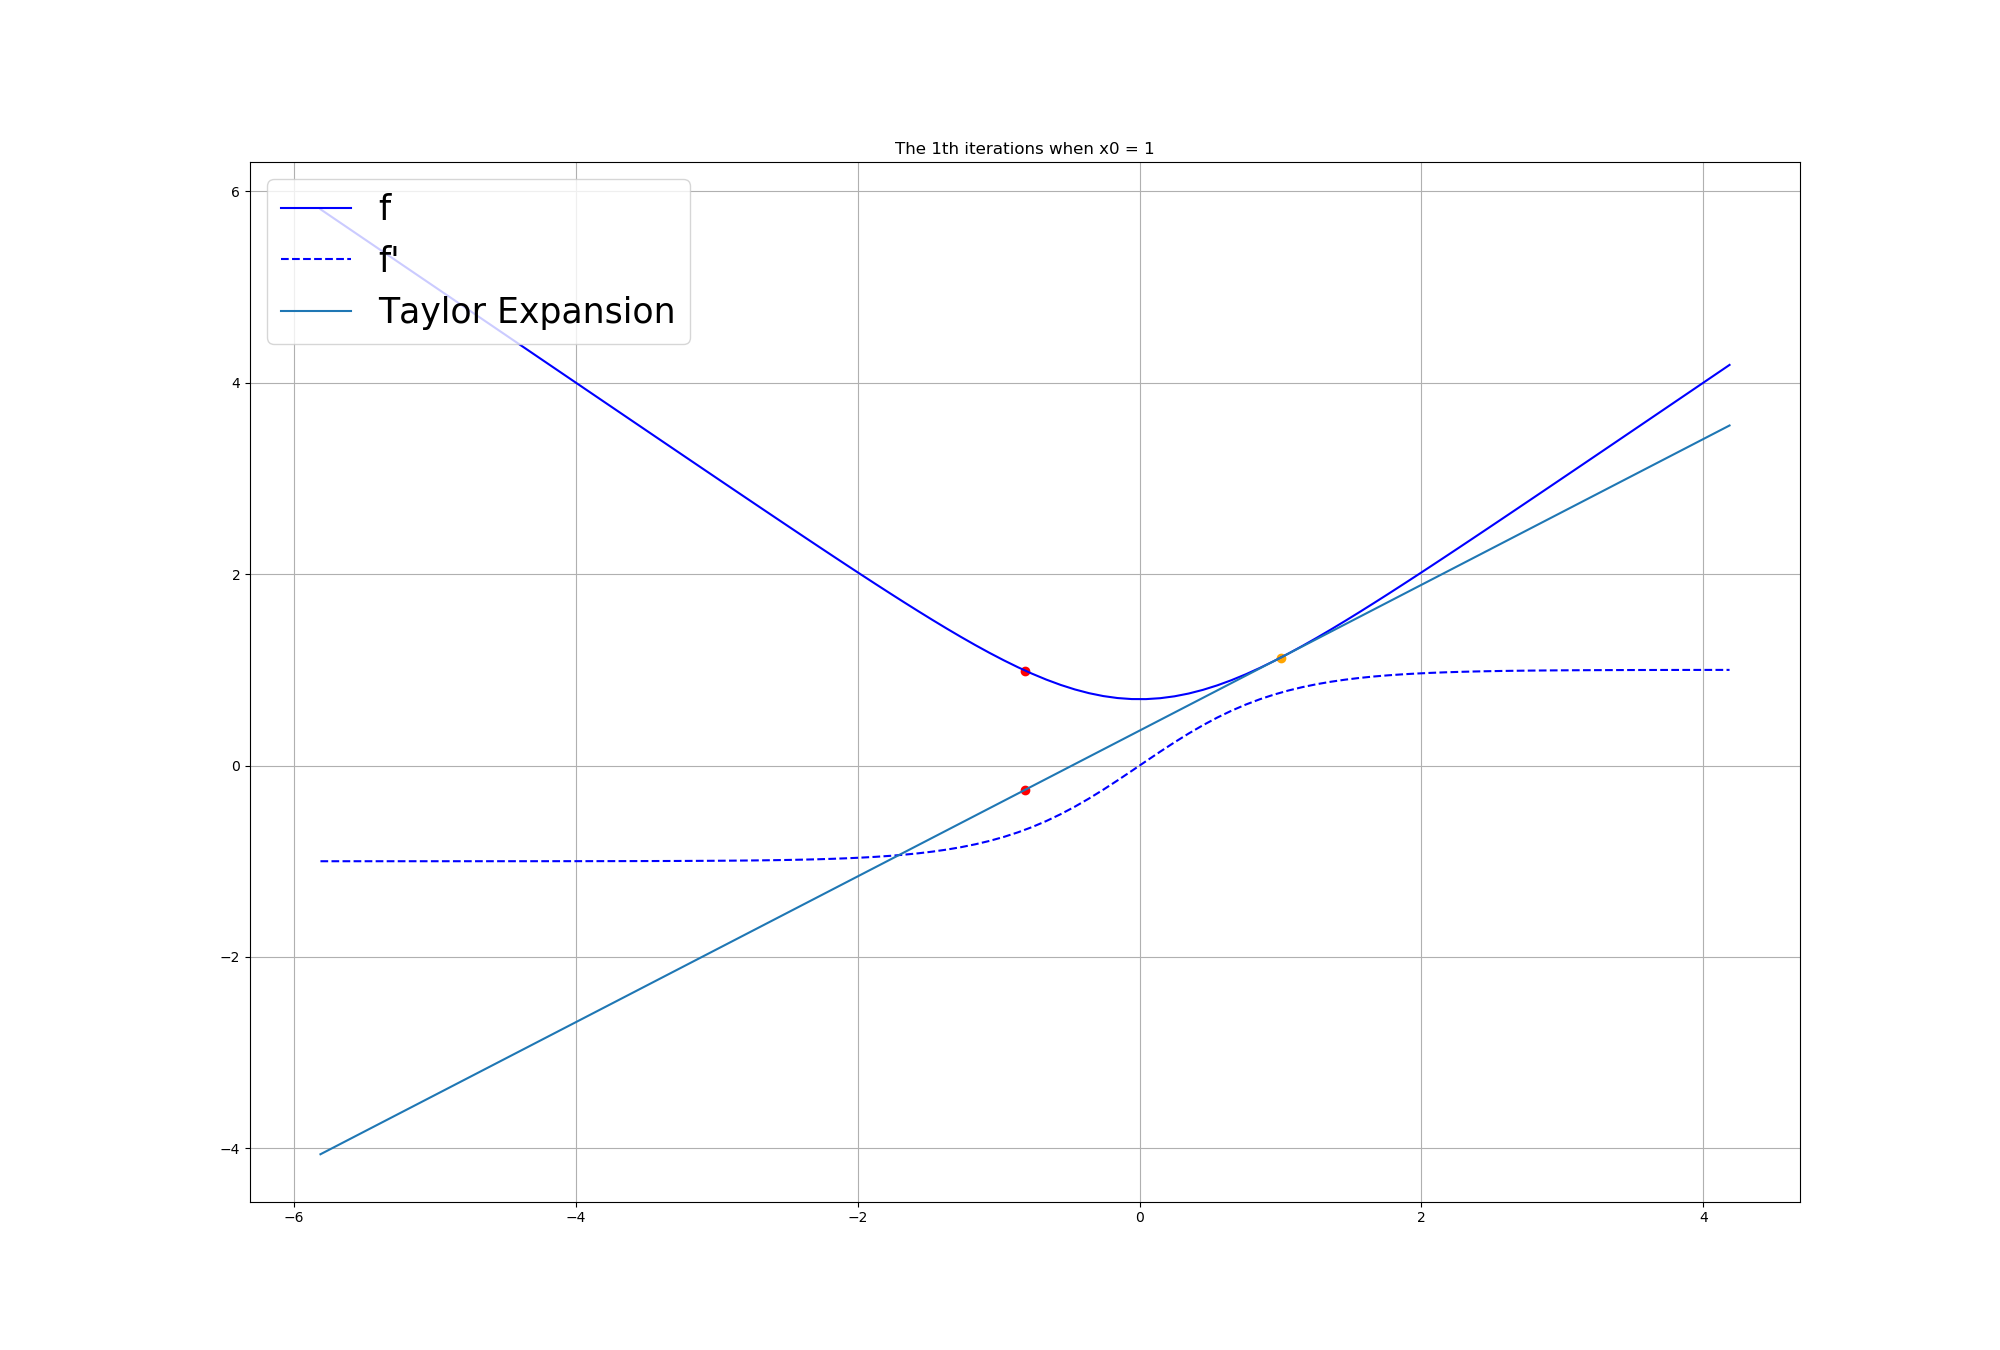
\includegraphics[scale=0.25]{f11.png}
    \end{figure}
    \begin{figure}[H]
        \centering
        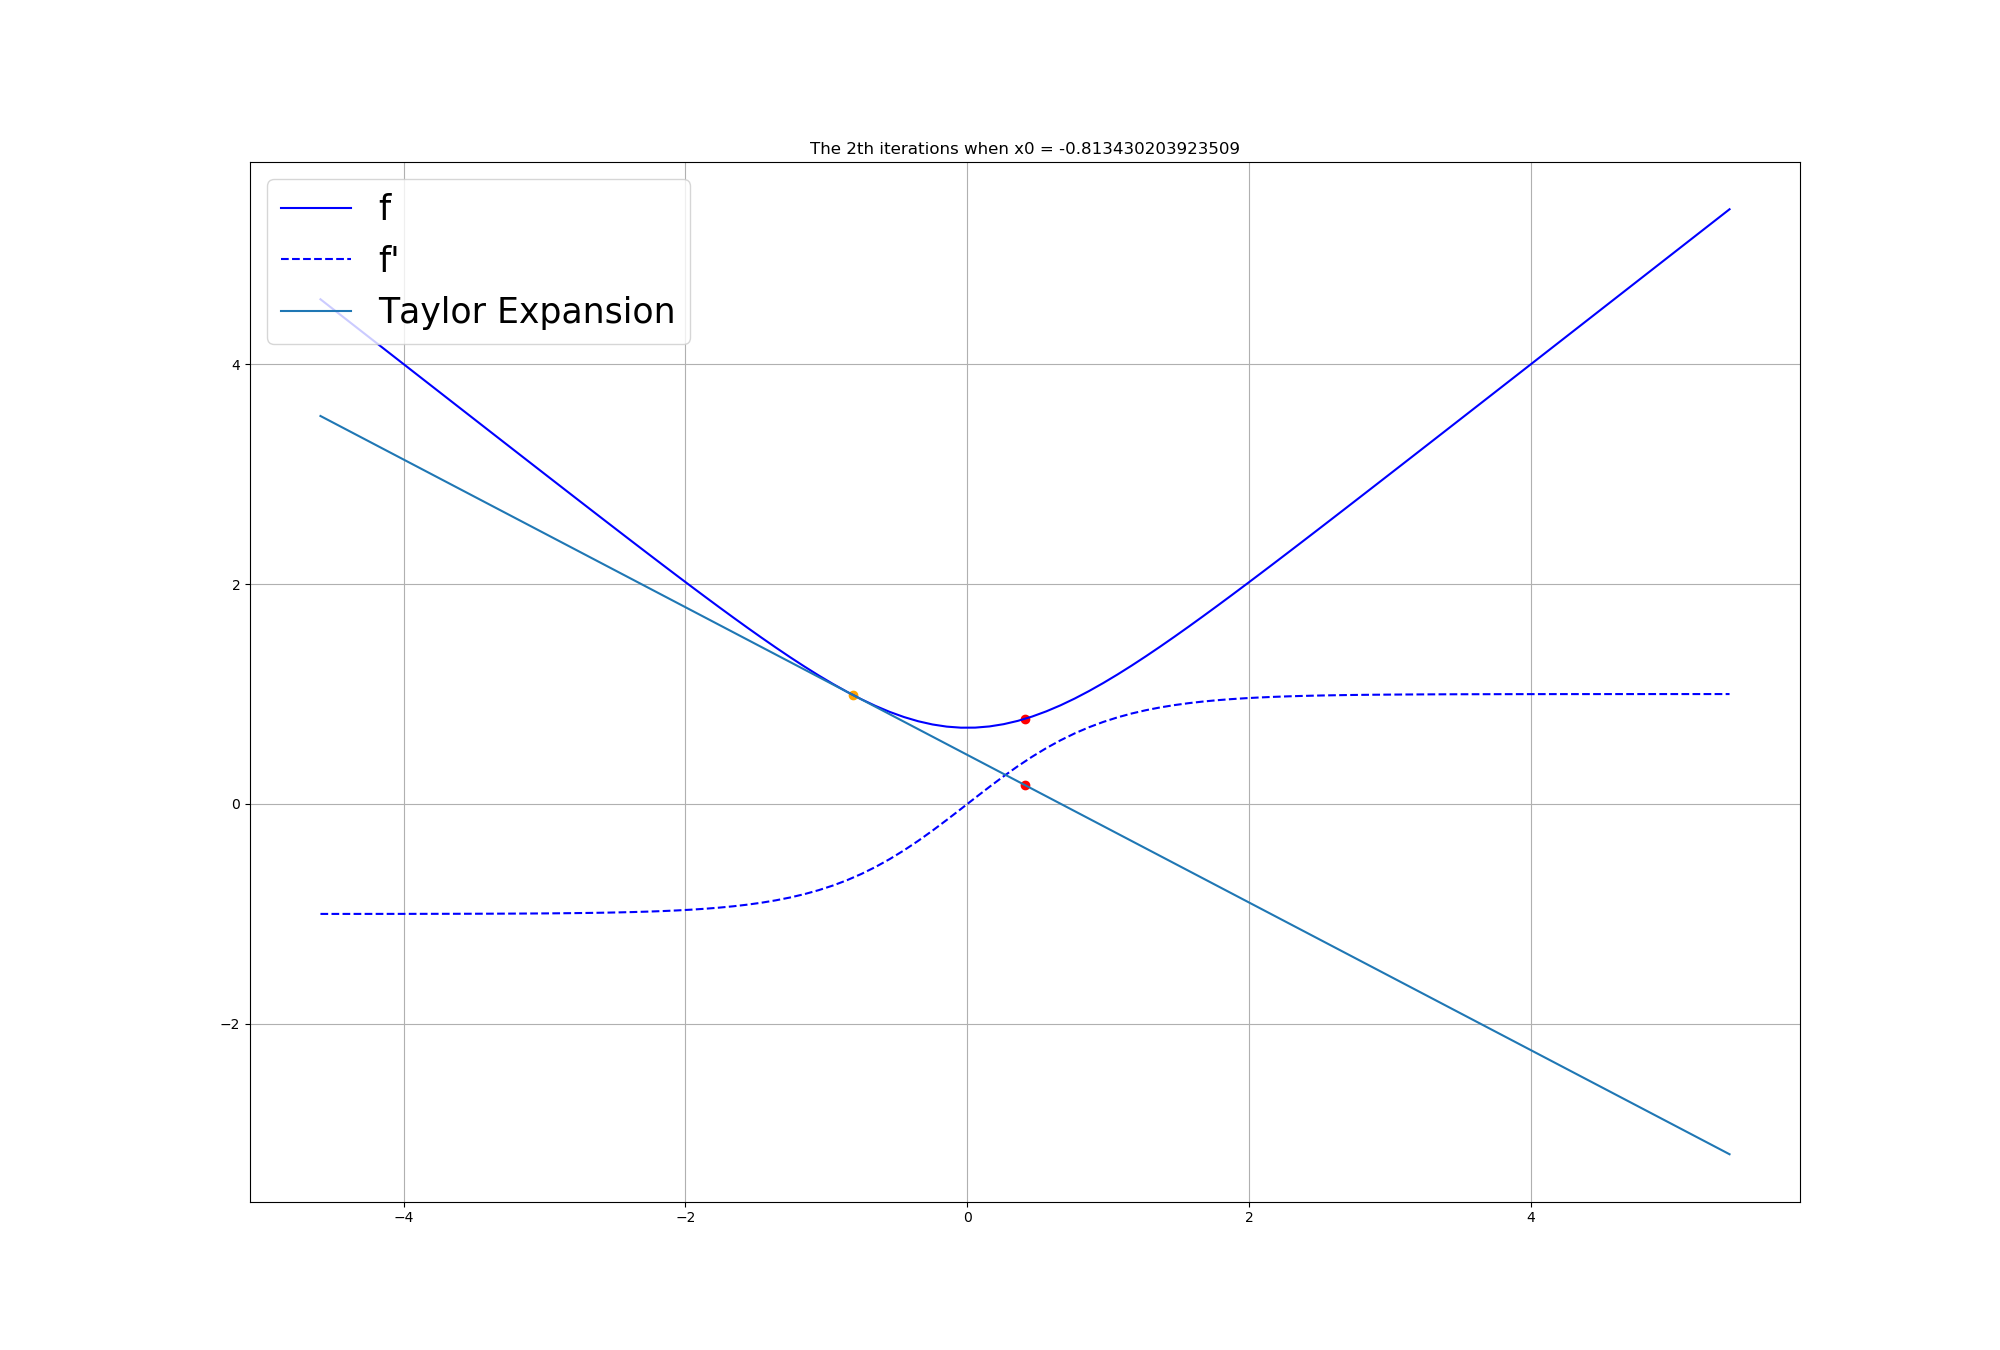
\includegraphics[scale=0.25]{f12.png}
    \end{figure}
    \begin{figure}[H]
        \centering
        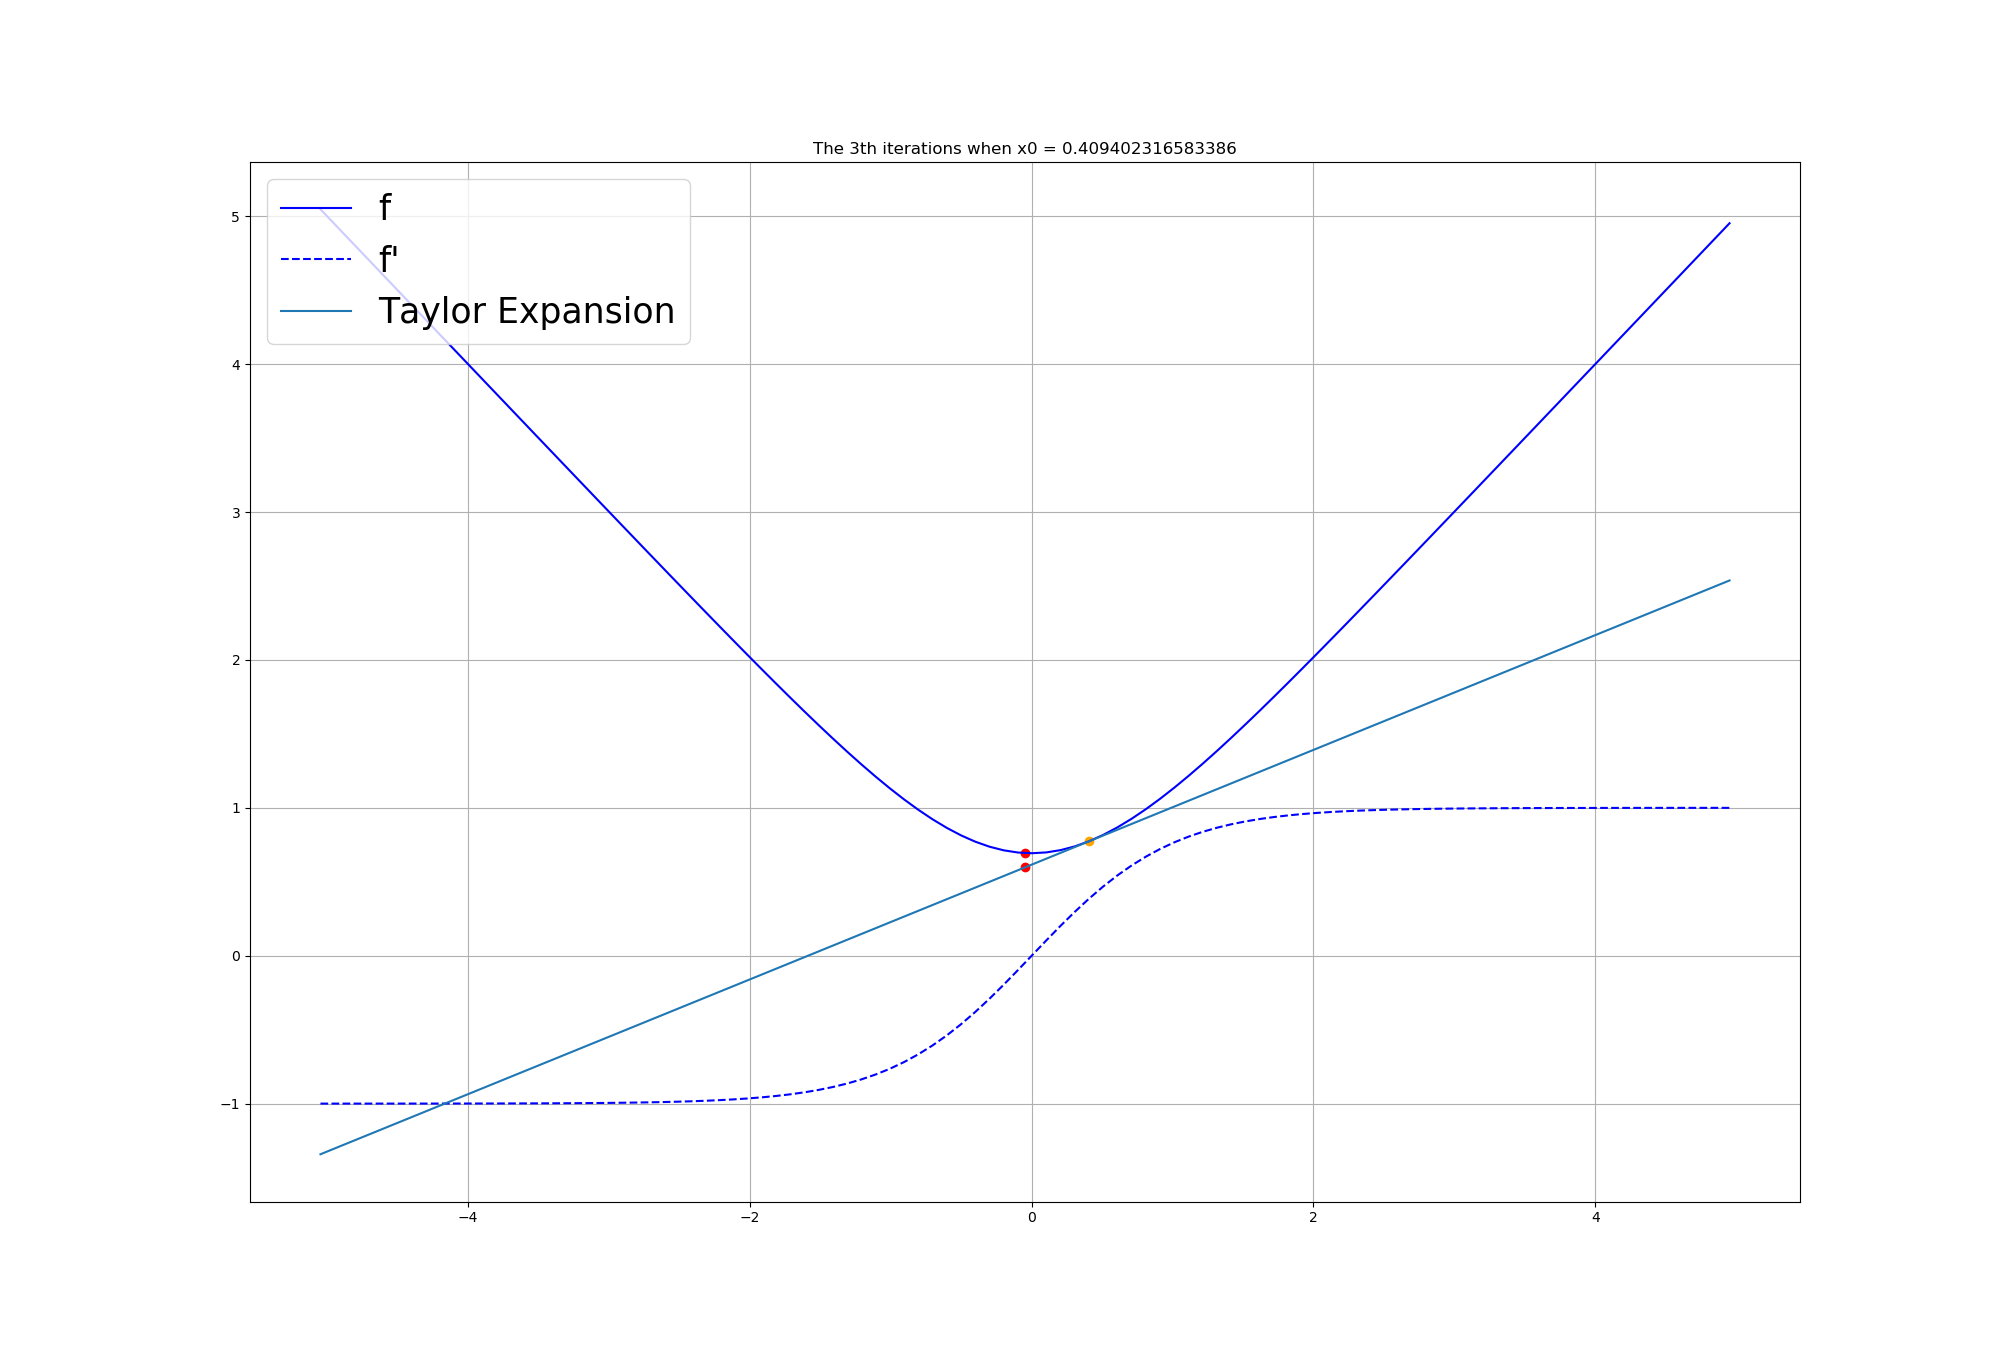
\includegraphics[scale=0.25]{f13.png}
    \end{figure}
    \begin{figure}[H]
        \centering
        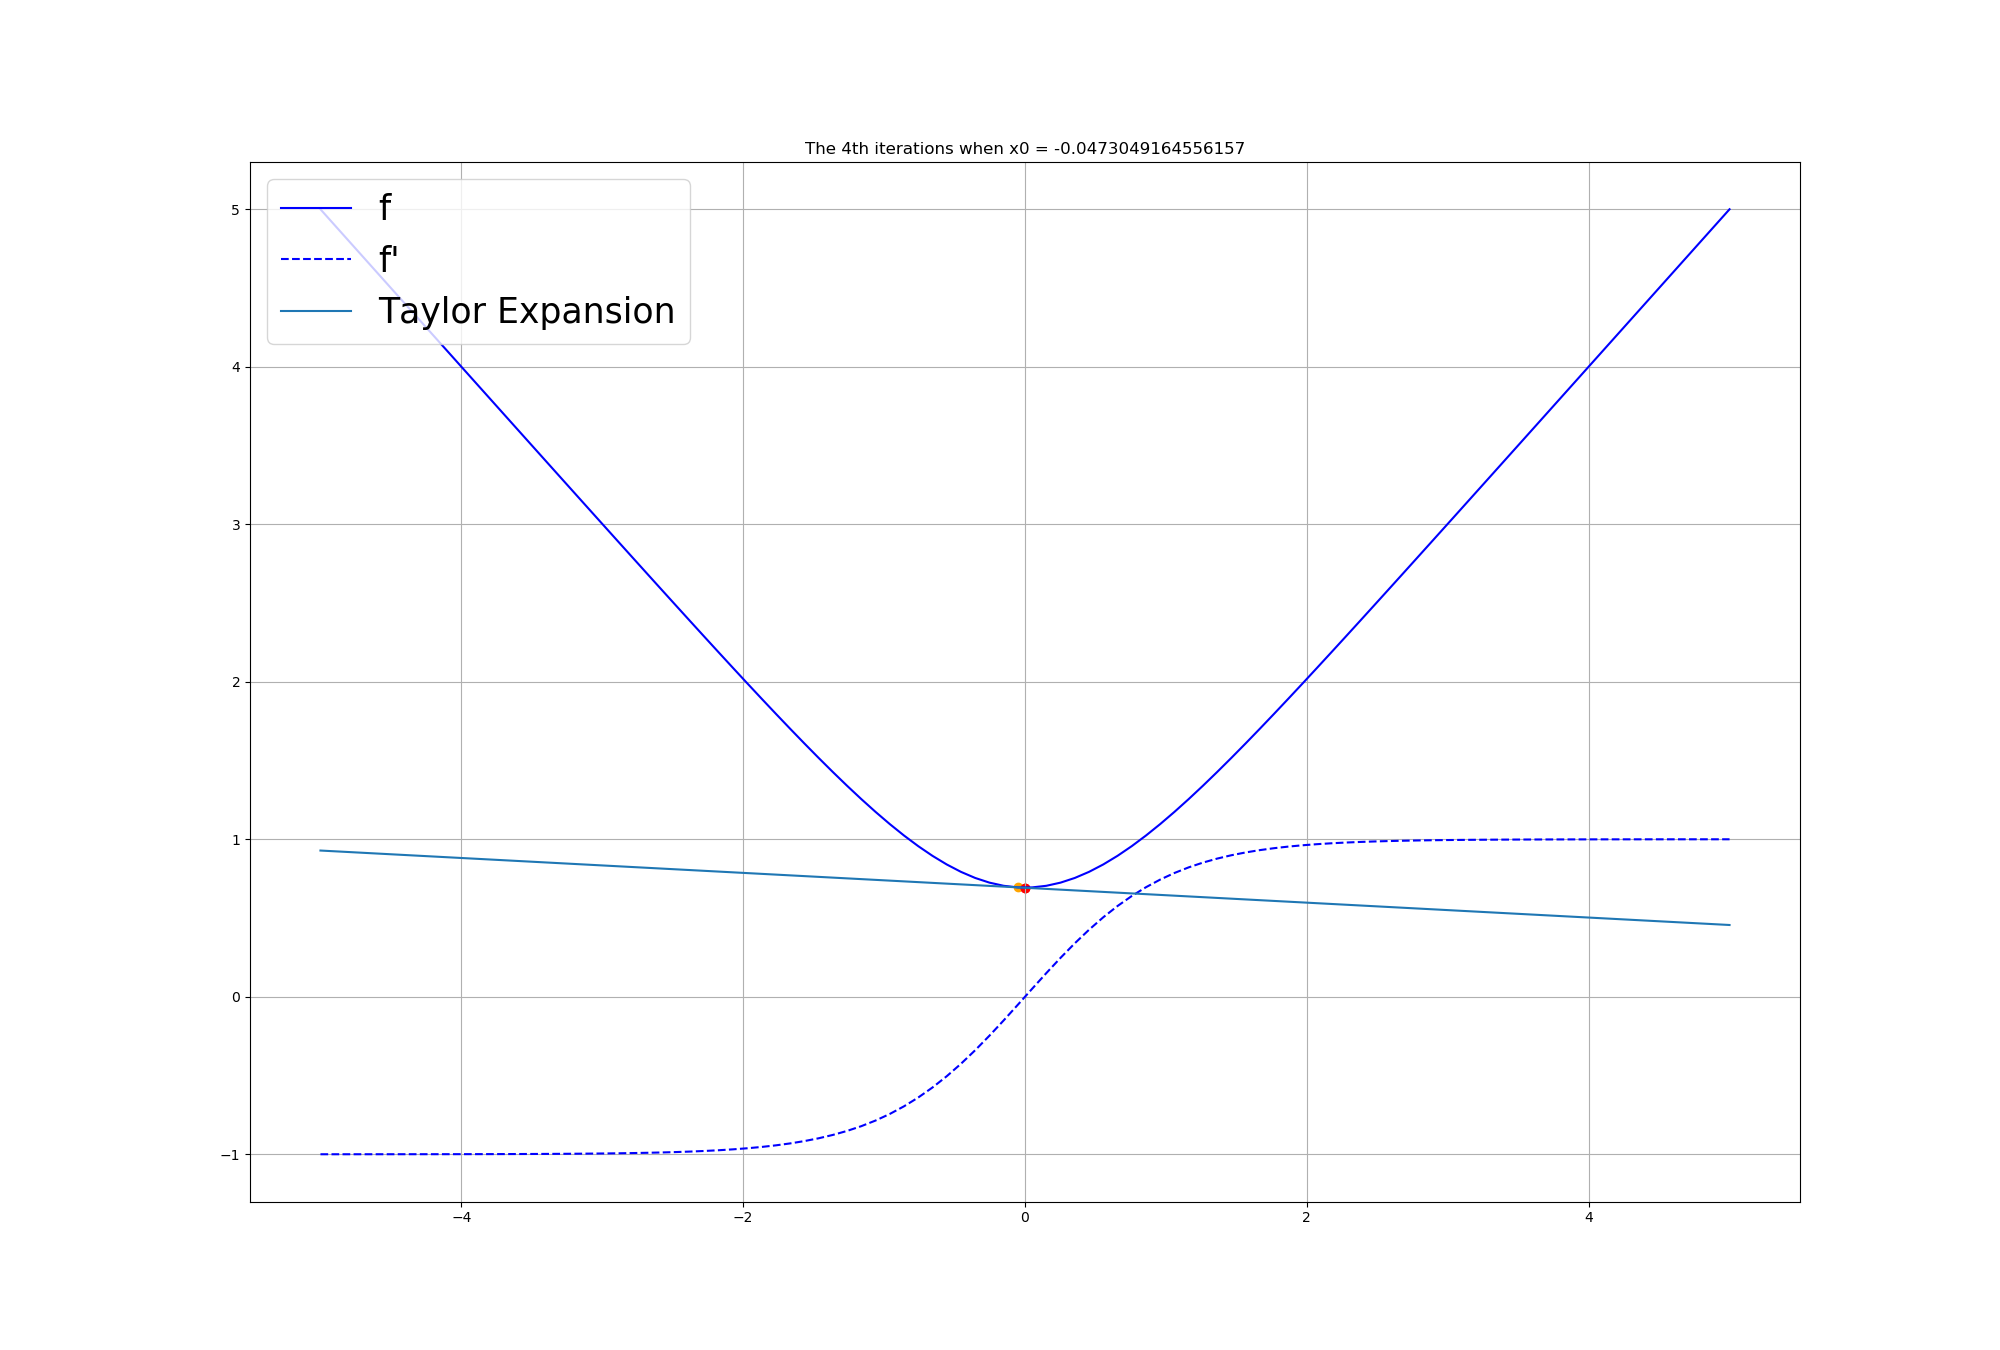
\includegraphics[scale=0.25]{f14.png}
    \end{figure}
    \begin{figure}[H]
        \centering
        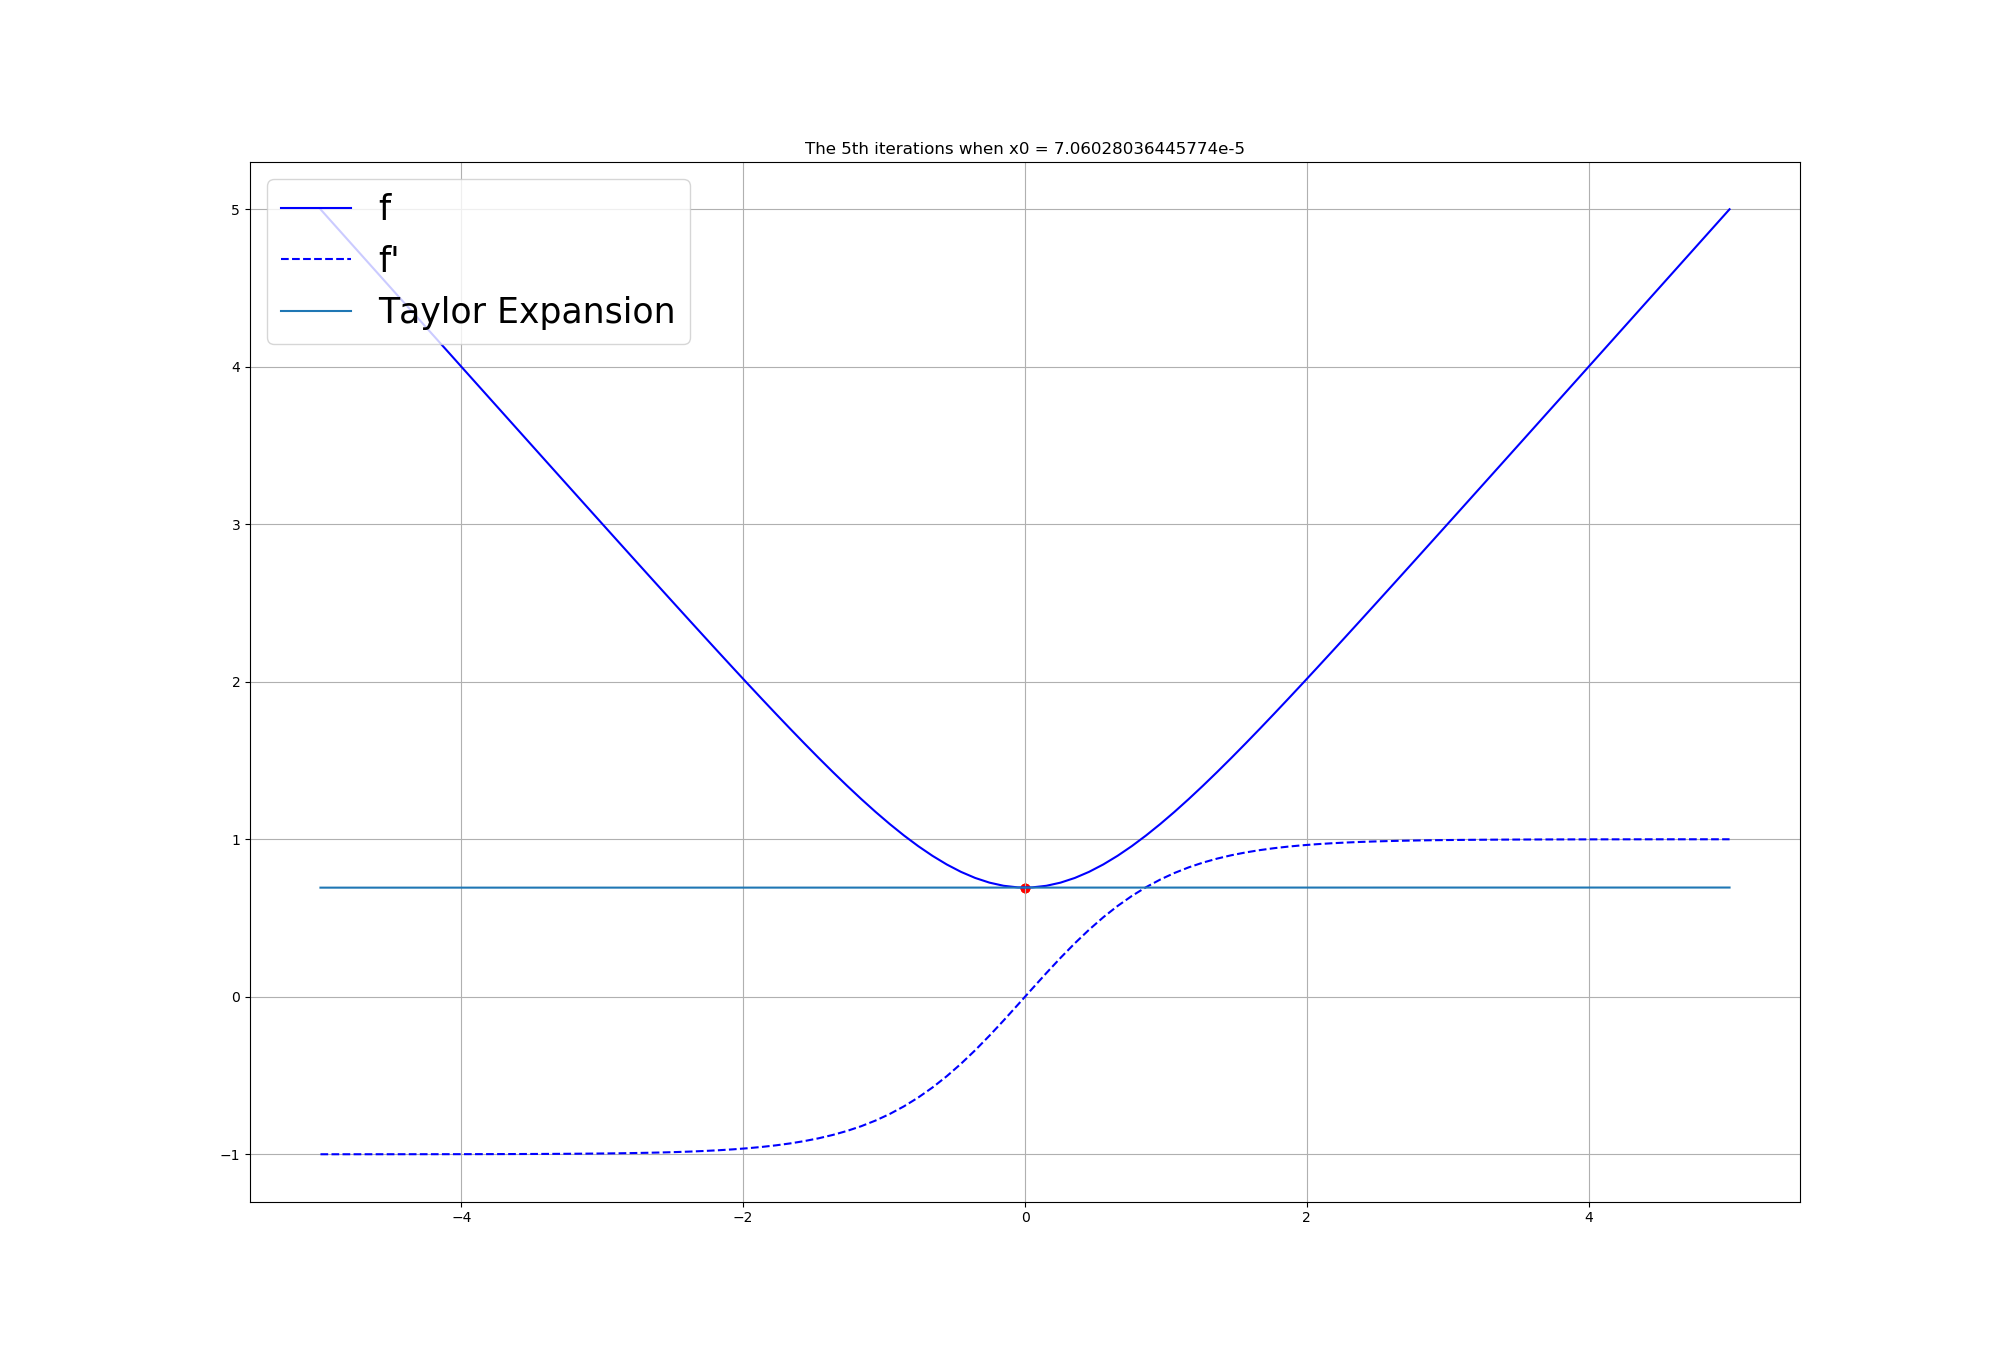
\includegraphics[scale=0.25]{f15.png}
    \end{figure}
    However, when $f(x)=\log(e^x+e^{-x}),x^{(0)} = 1.1,t = 1$, we can find $x$ is farther from the minimize point after each iteration, its absolute value also grows larger.
    \begin{figure}[H]
        \centering
        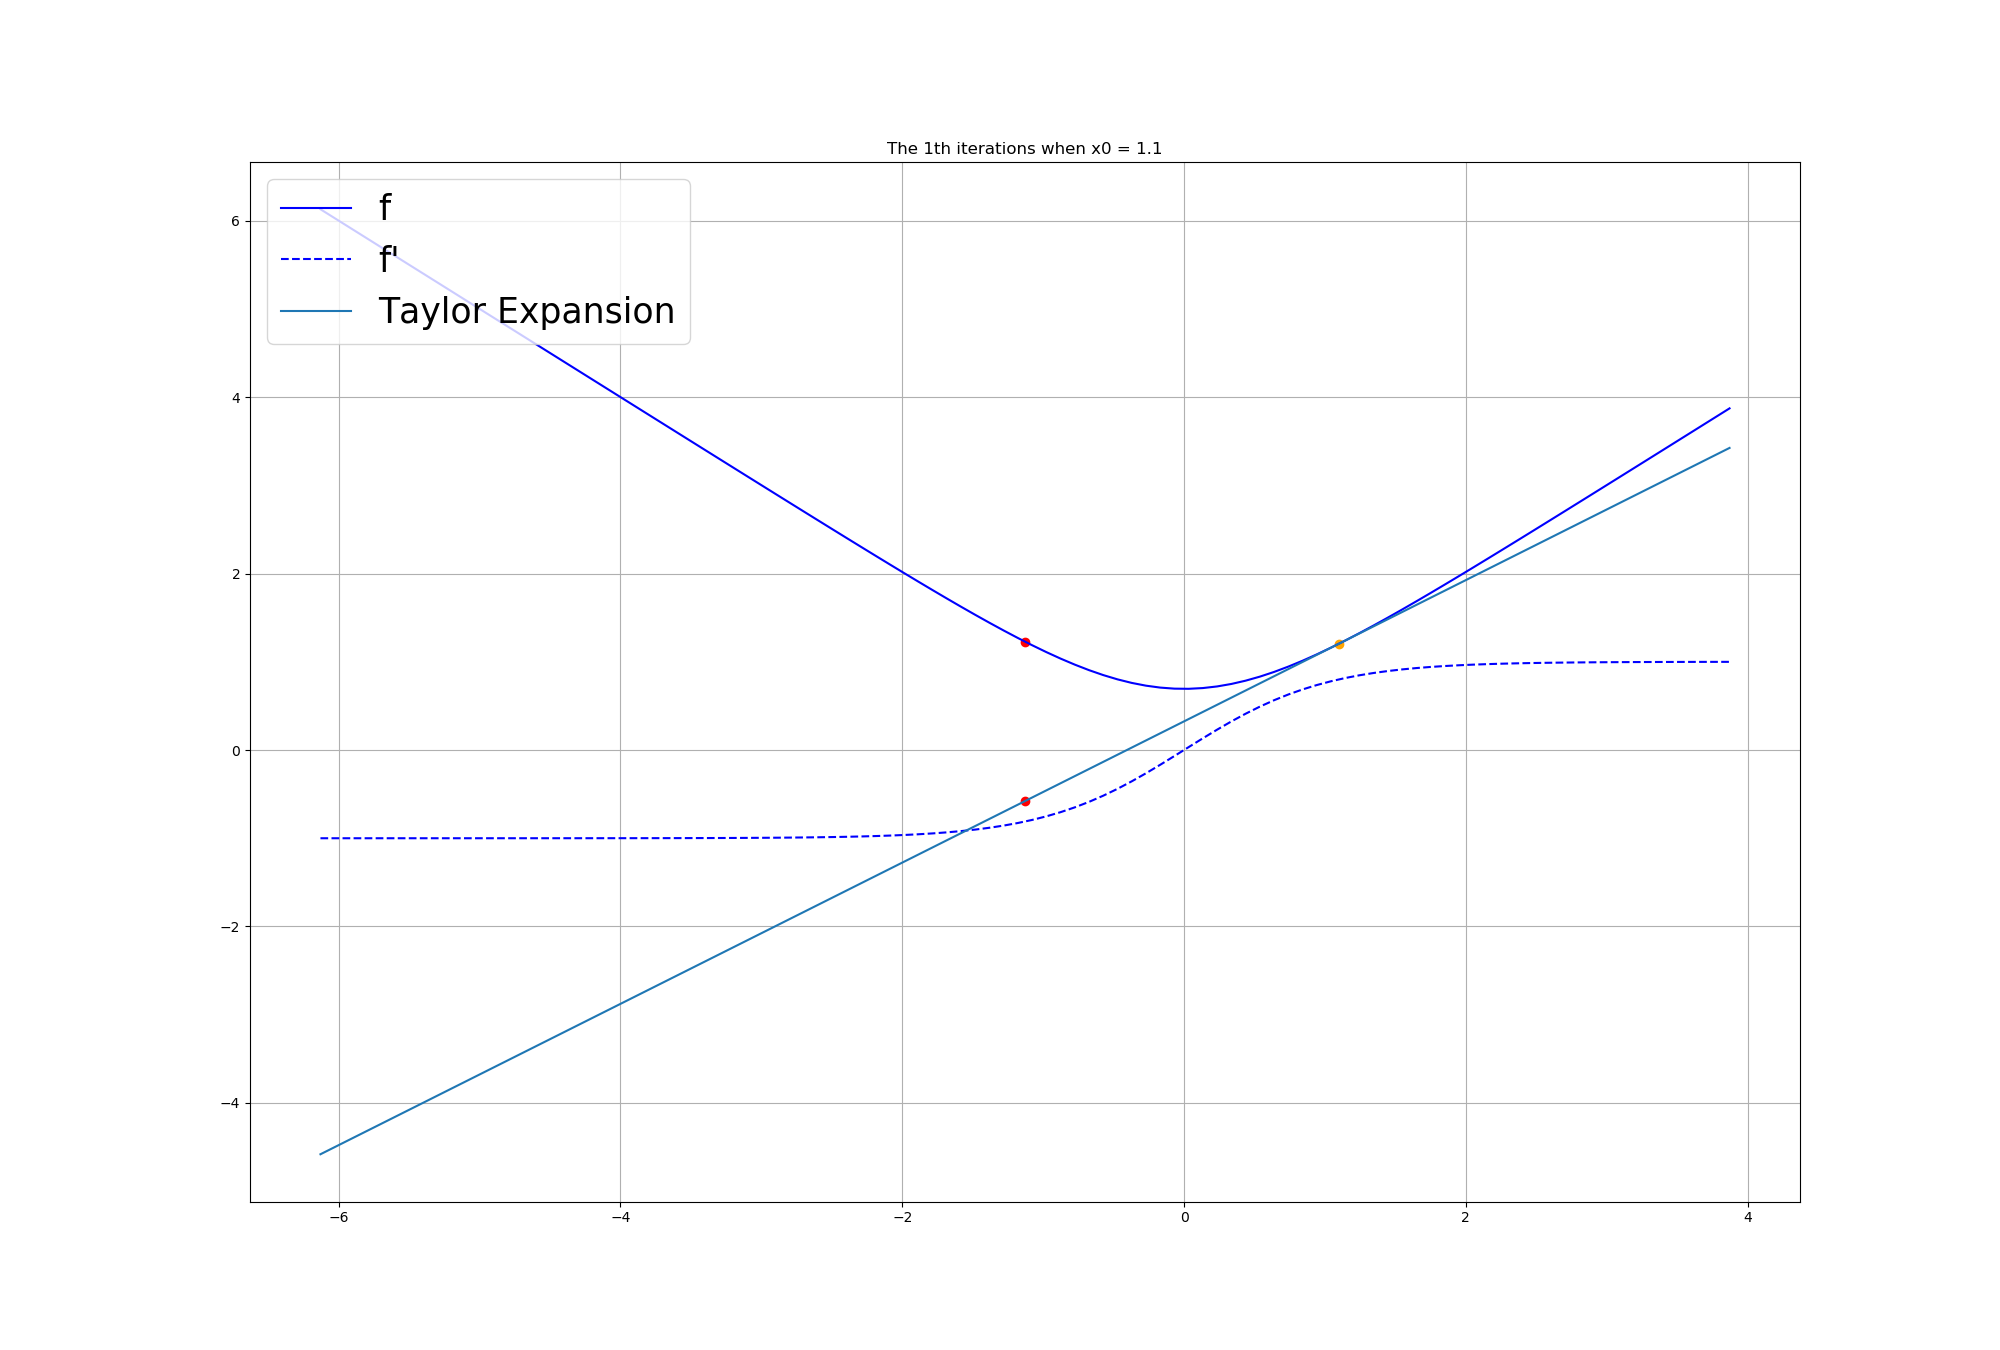
\includegraphics[scale=0.25]{f21.png}
    \end{figure}
    \begin{figure}[H]
        \centering
        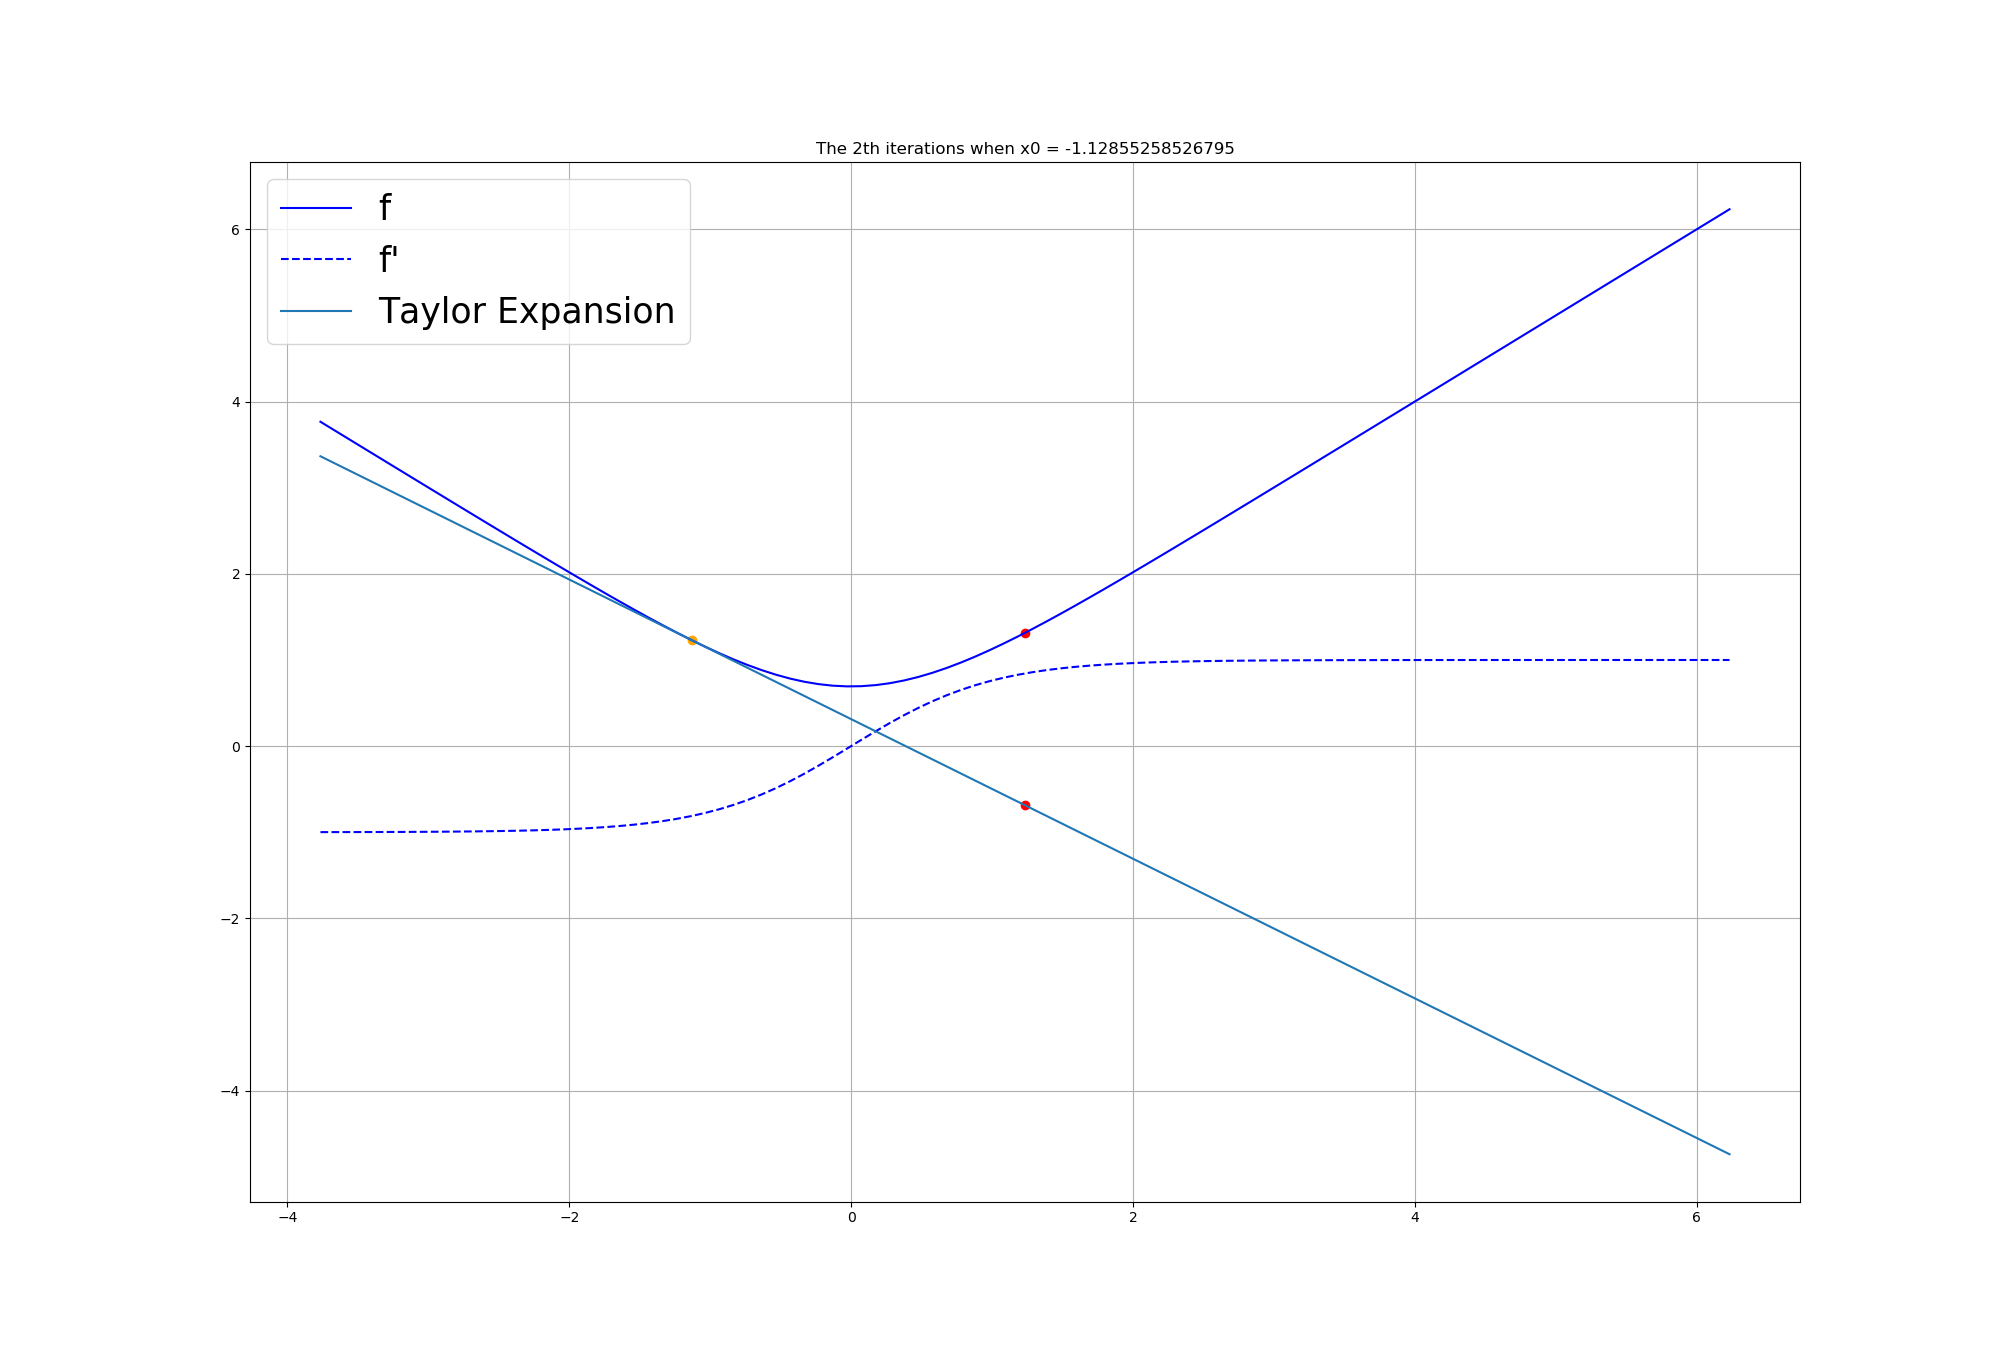
\includegraphics[scale=0.25]{f22.png}
    \end{figure}
    \begin{figure}[H]
        \centering
        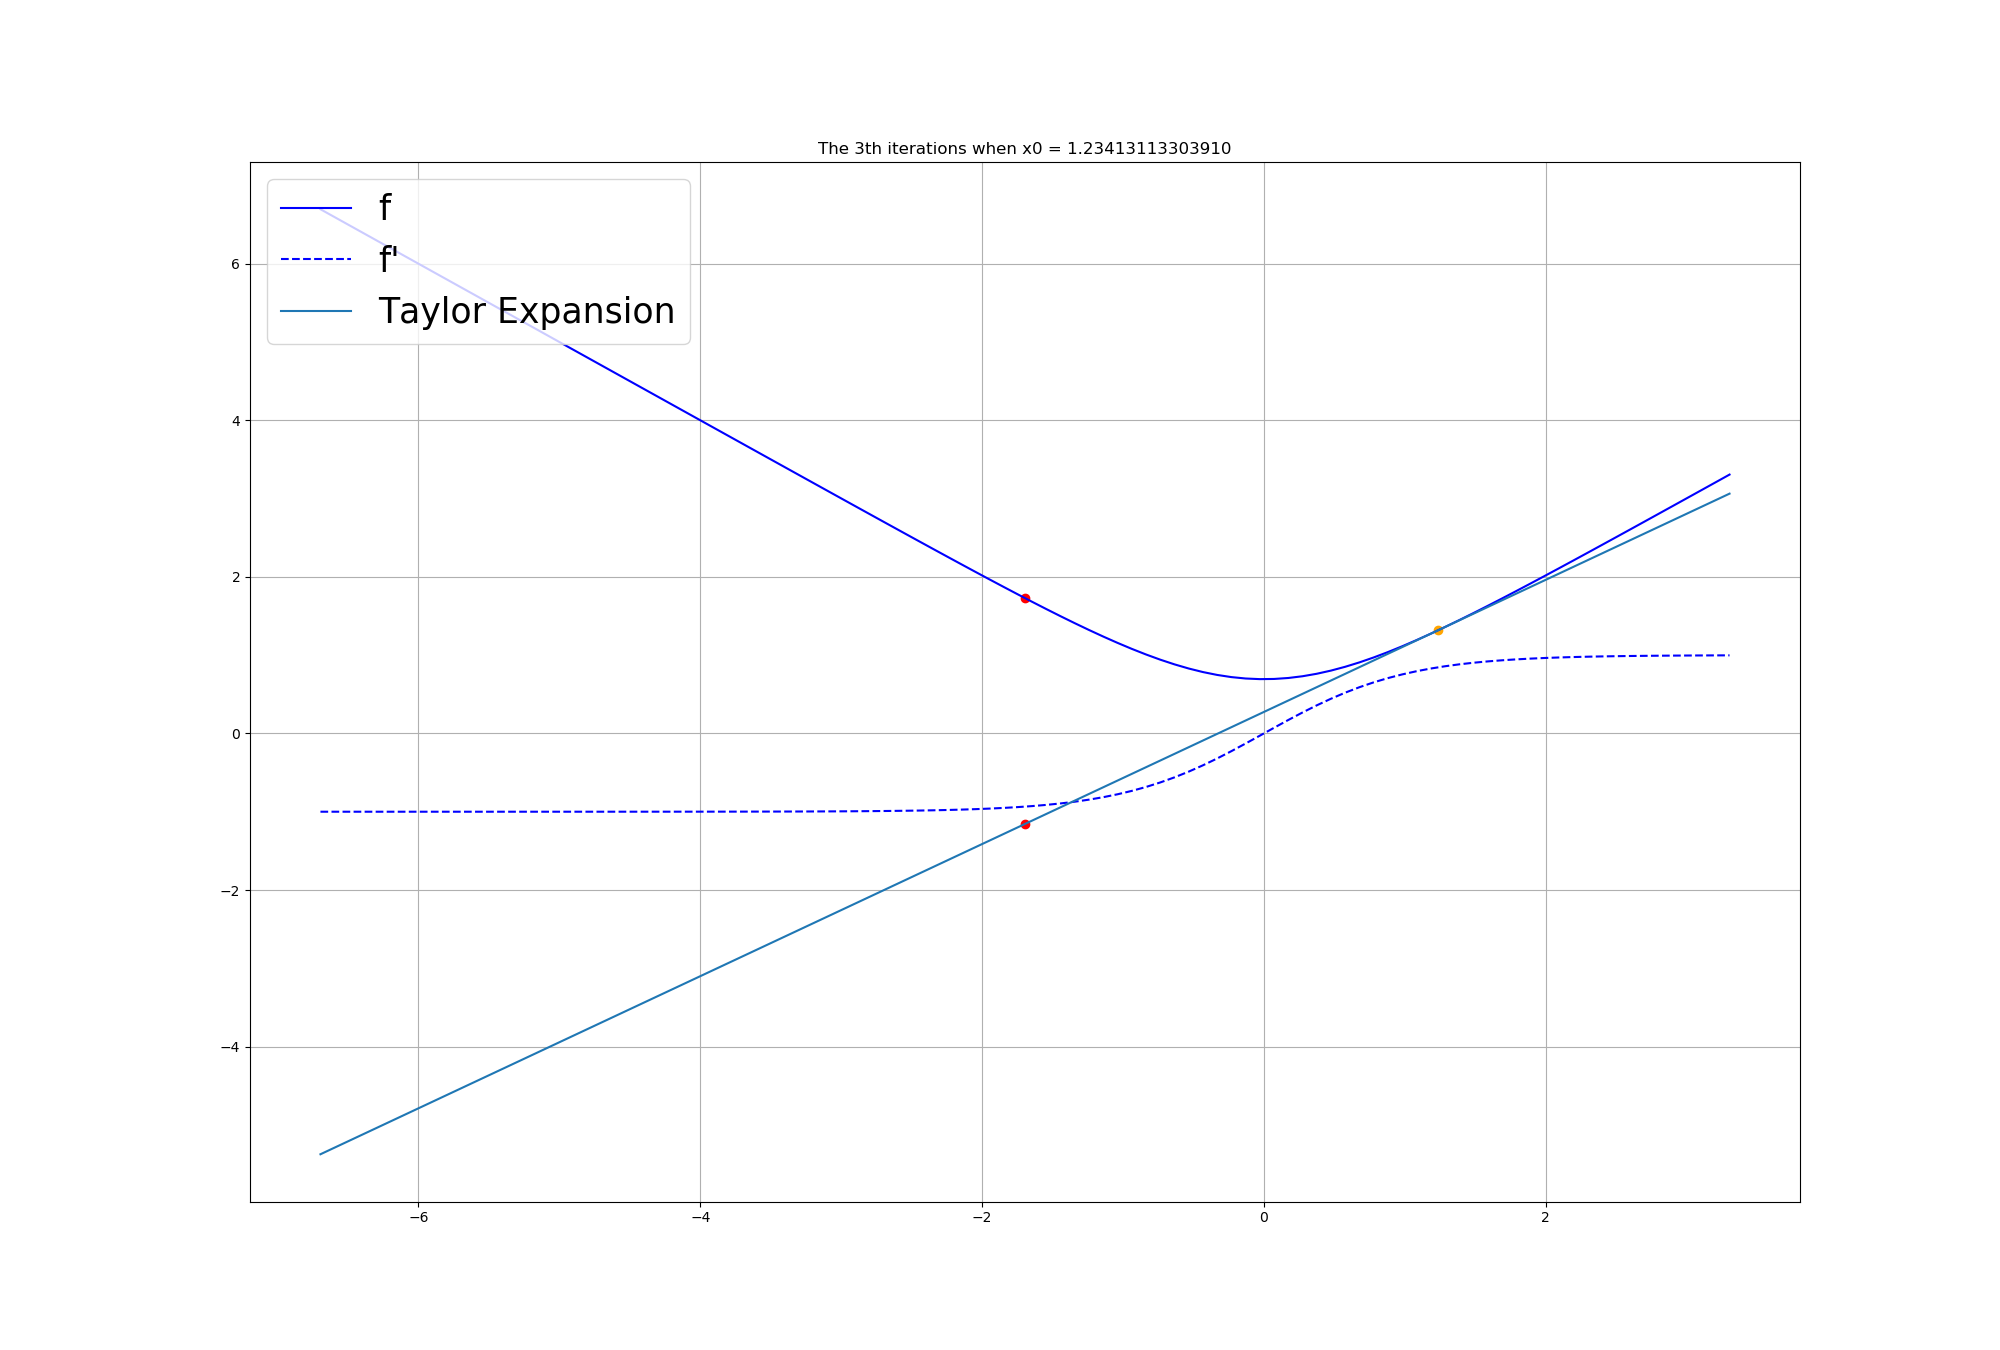
\includegraphics[scale=0.25]{f23.png}
    \end{figure}
    \begin{figure}[H]
        \centering
        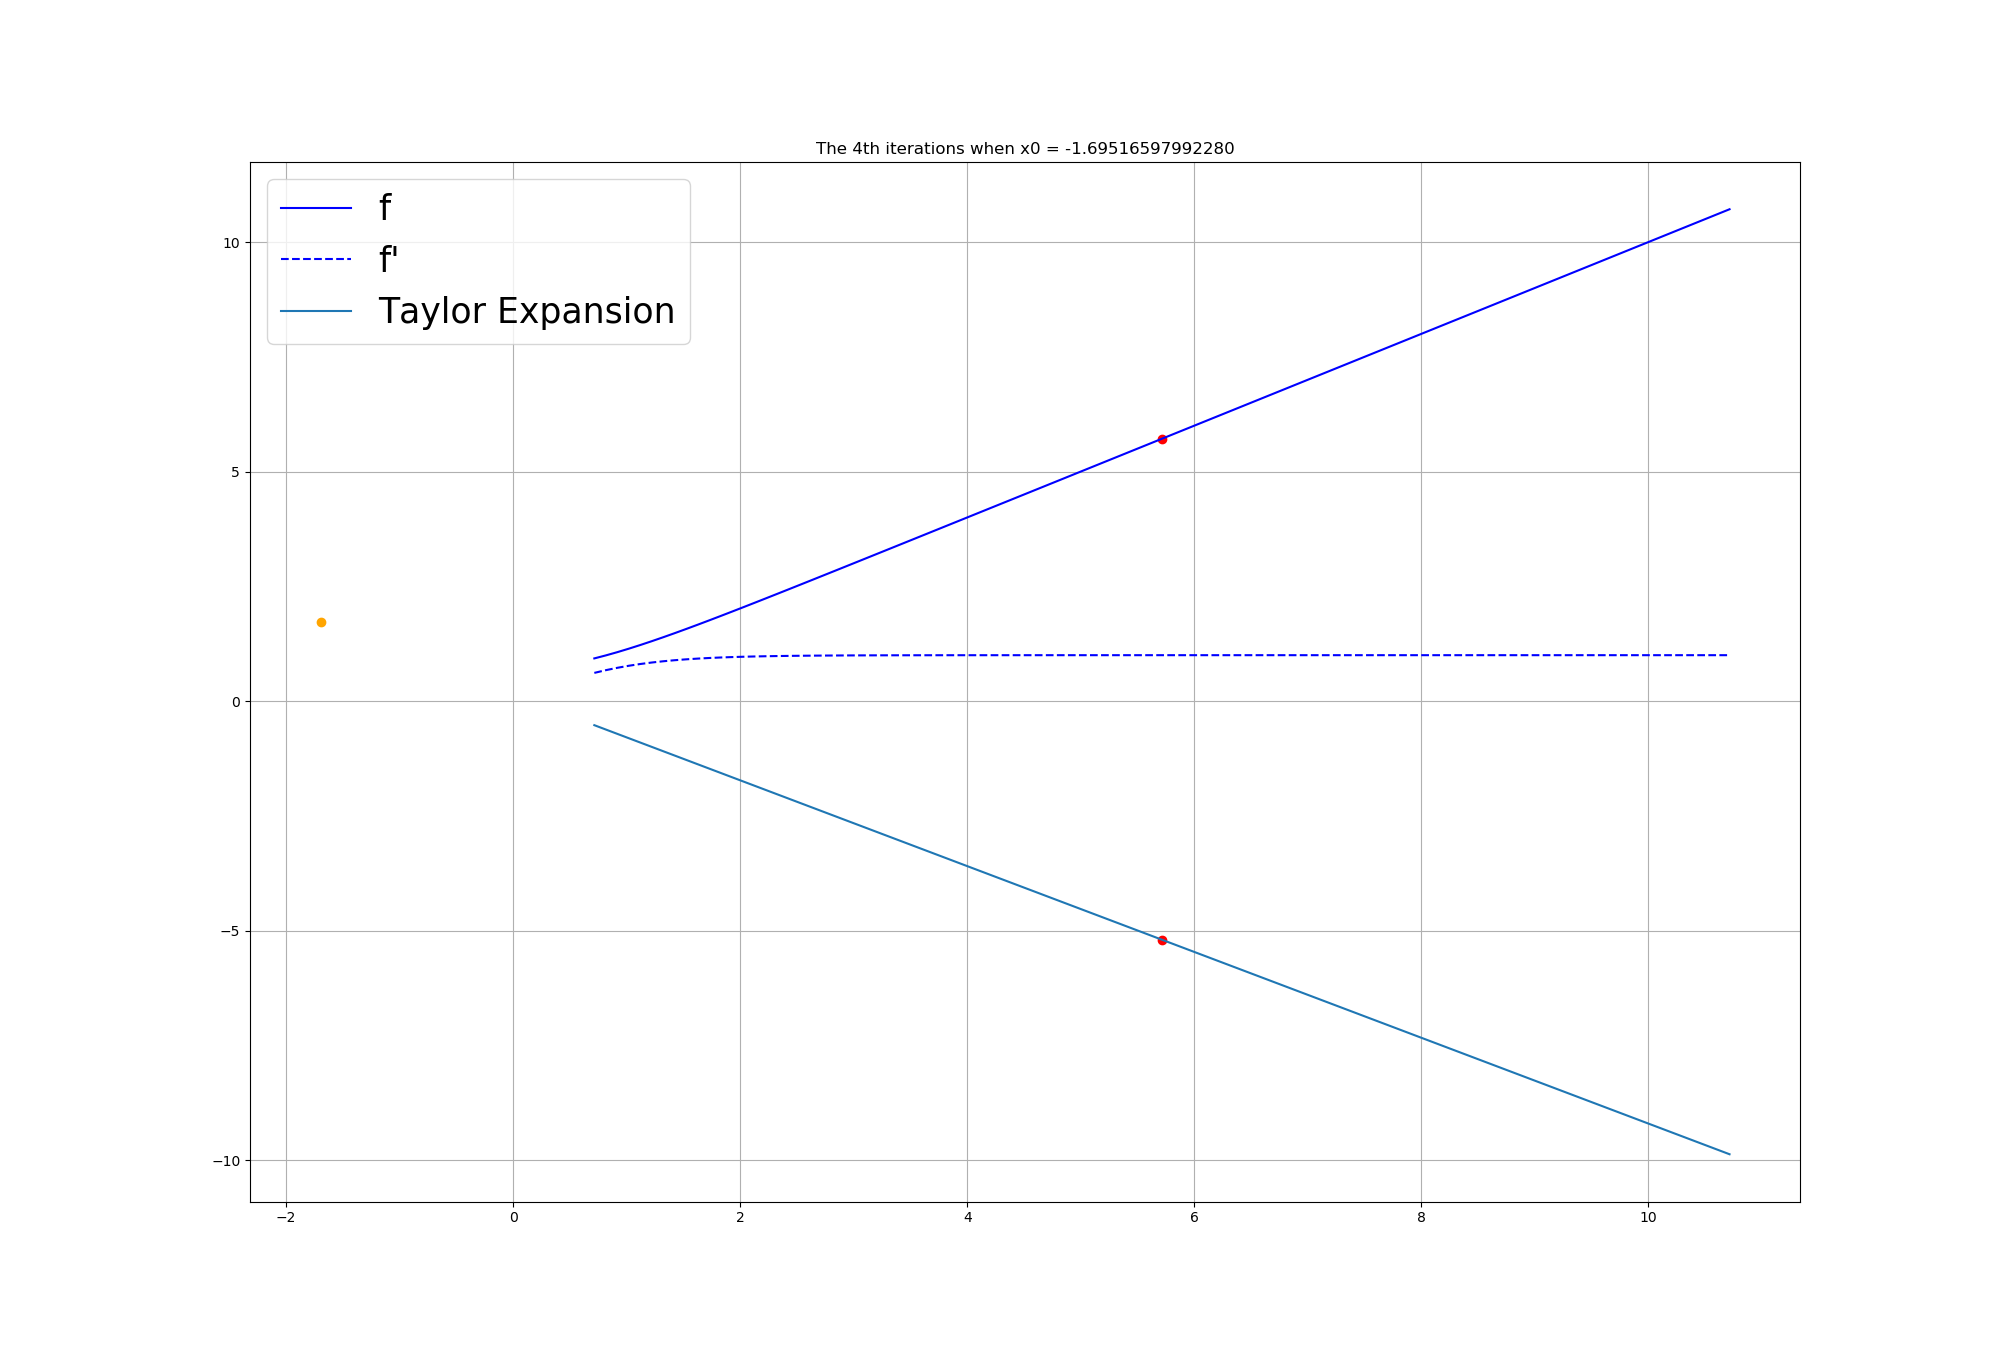
\includegraphics[scale=0.25]{f24.png}
    \end{figure}
    \begin{figure}[H]
        \centering
        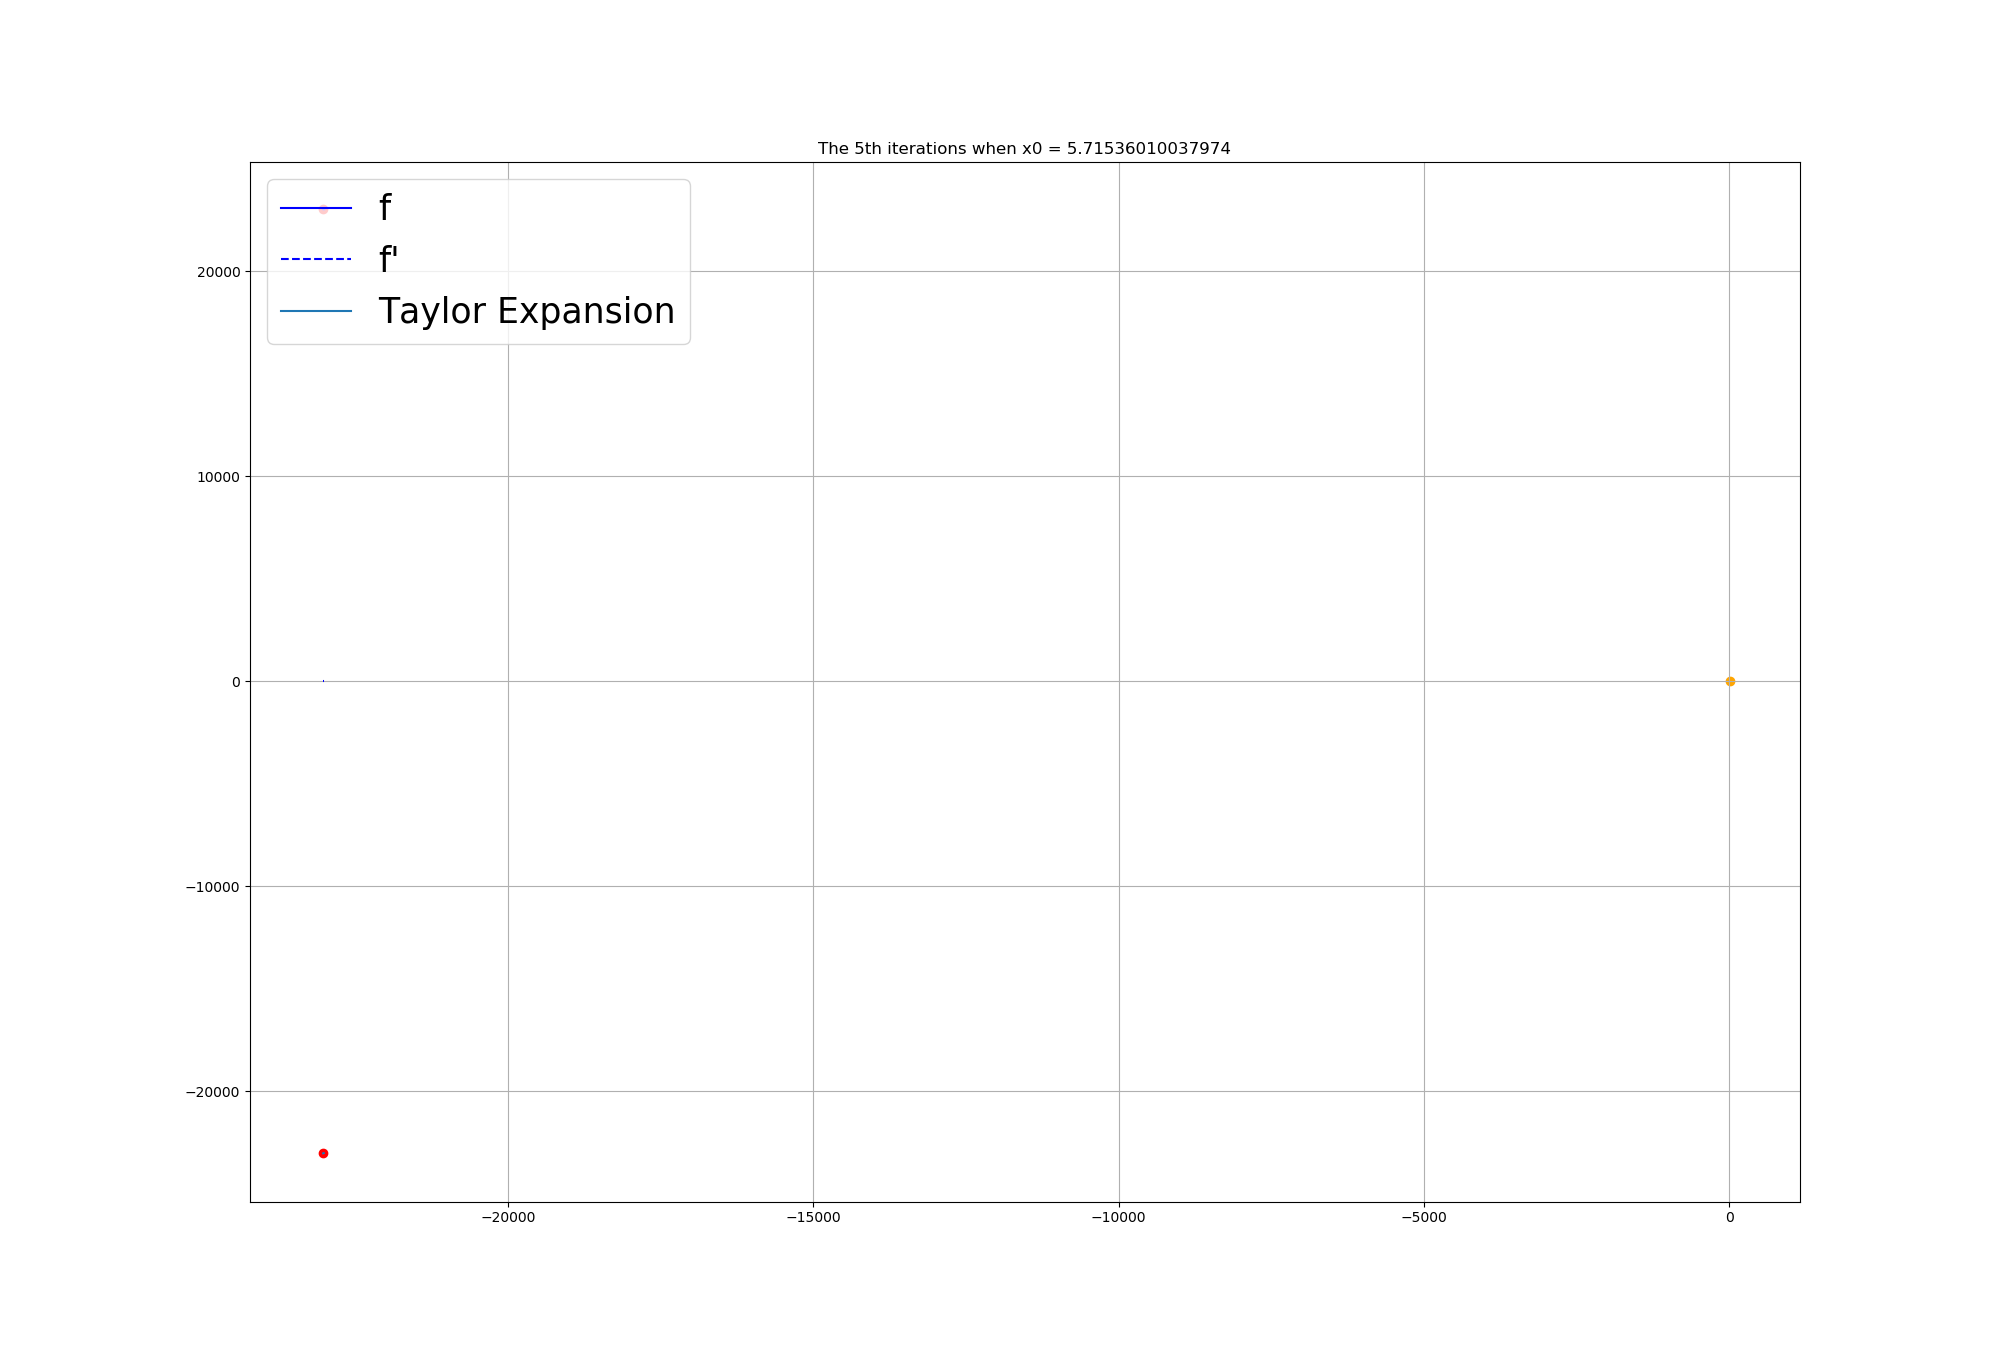
\includegraphics[scale=0.25]{f25.png}
    \end{figure}
    \item When $f(x)=-\log x+x,x^{(0)} = 3,t = 1$, we can find after the first iteration, $x^{(1)}=3-\frac{1-1/3}{1/9}=-3$, which is not in $f(x)$ \dom, so the process has to be interrupted.
    \begin{figure}[H]
        \centering
        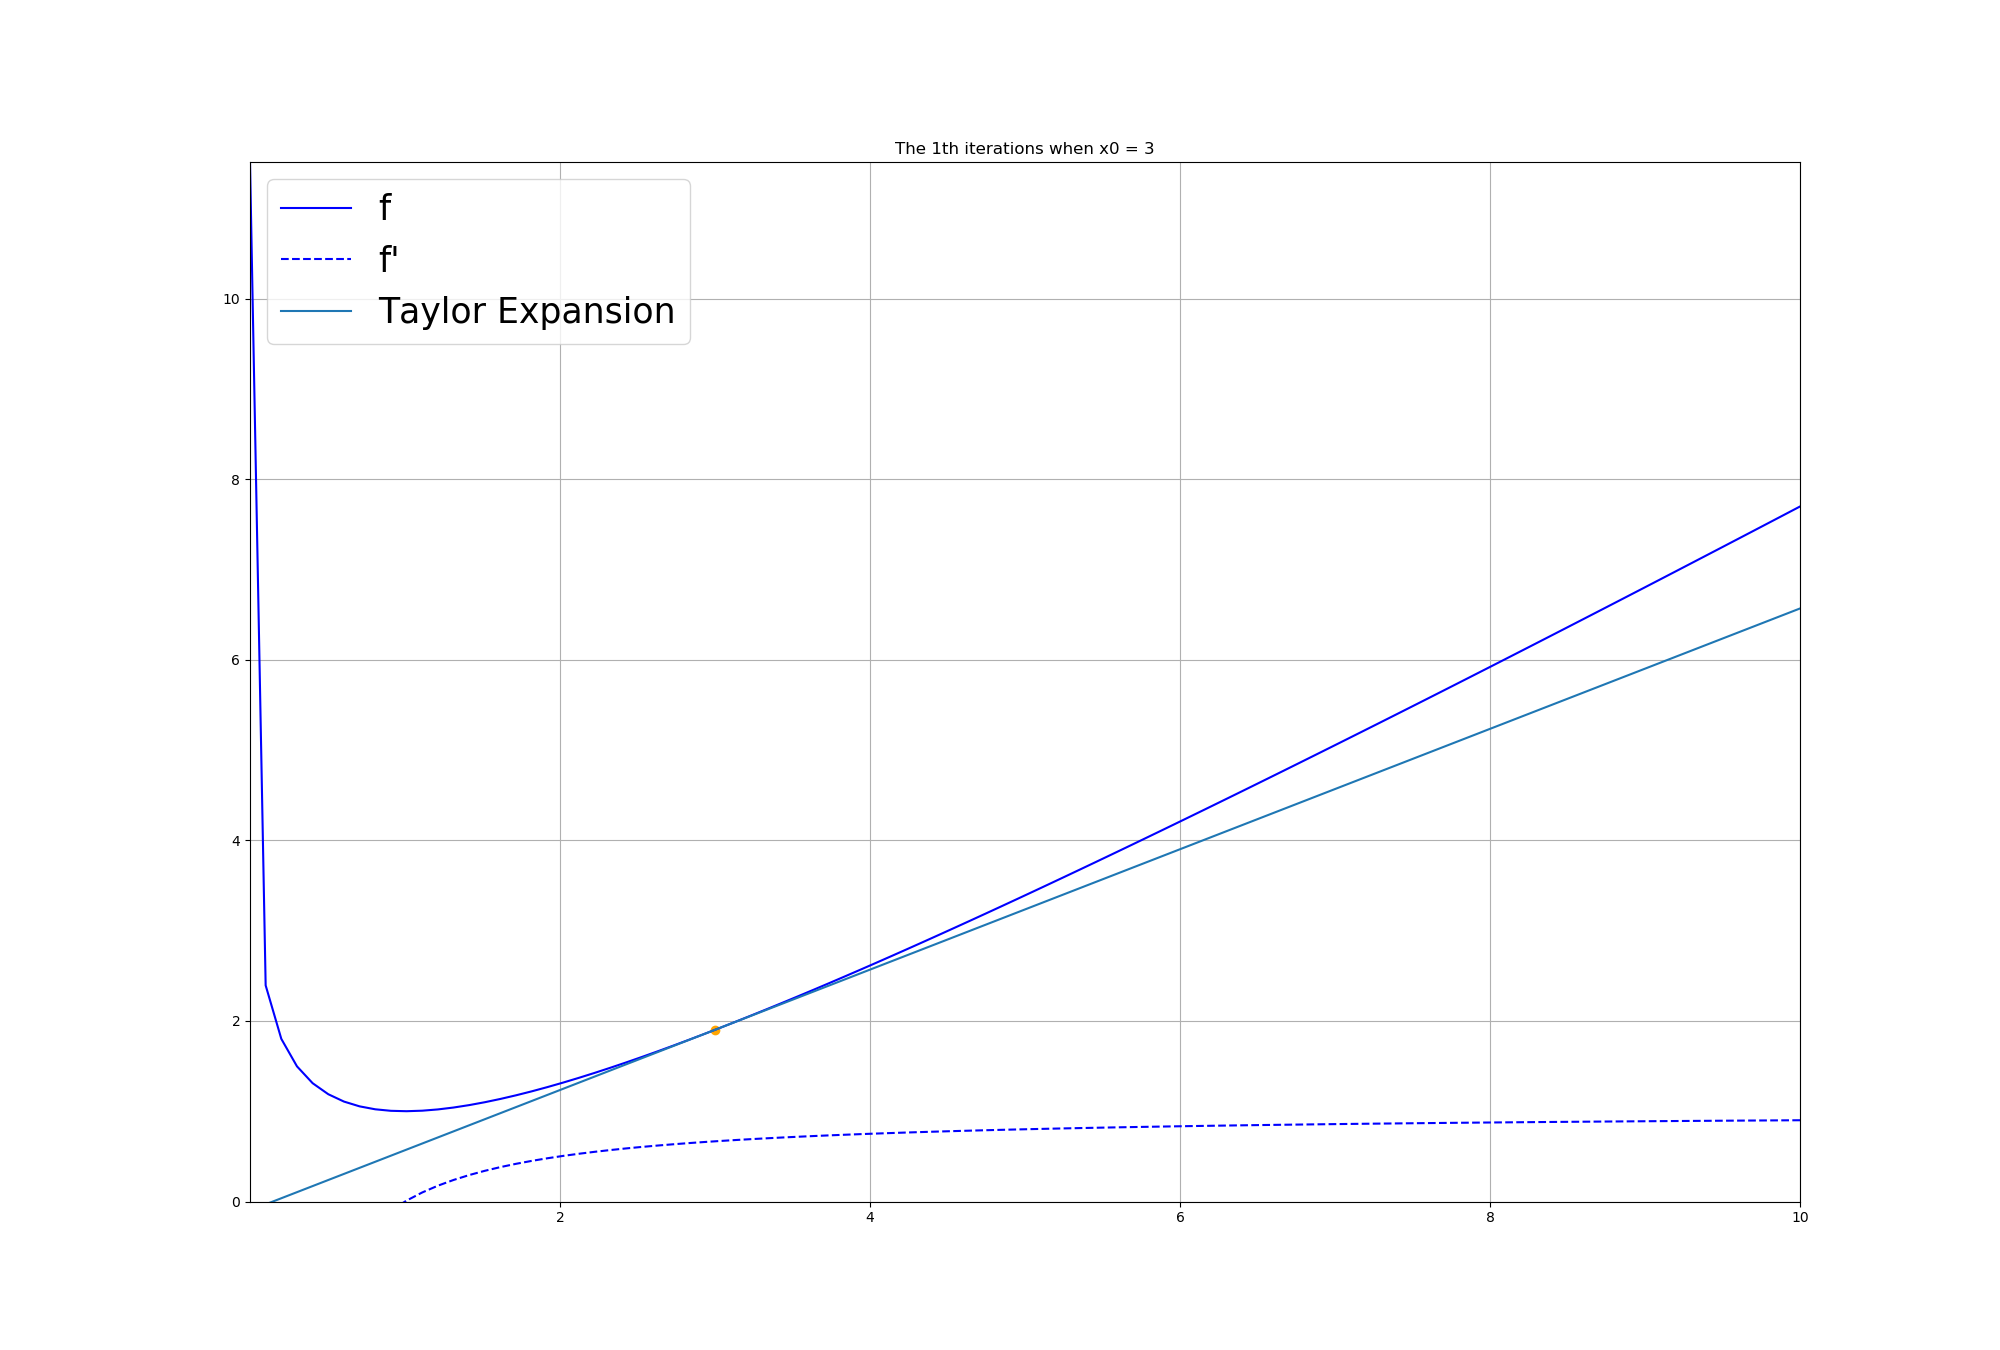
\includegraphics[scale=0.25]{f31.png}
    \end{figure}
    However, if I change $x^{(0)}$'s value to 1.9, the \textbf{\emph{Newton Method}} still converges to the minimize point $x=1$
    \begin{figure}[H]
        \centering
        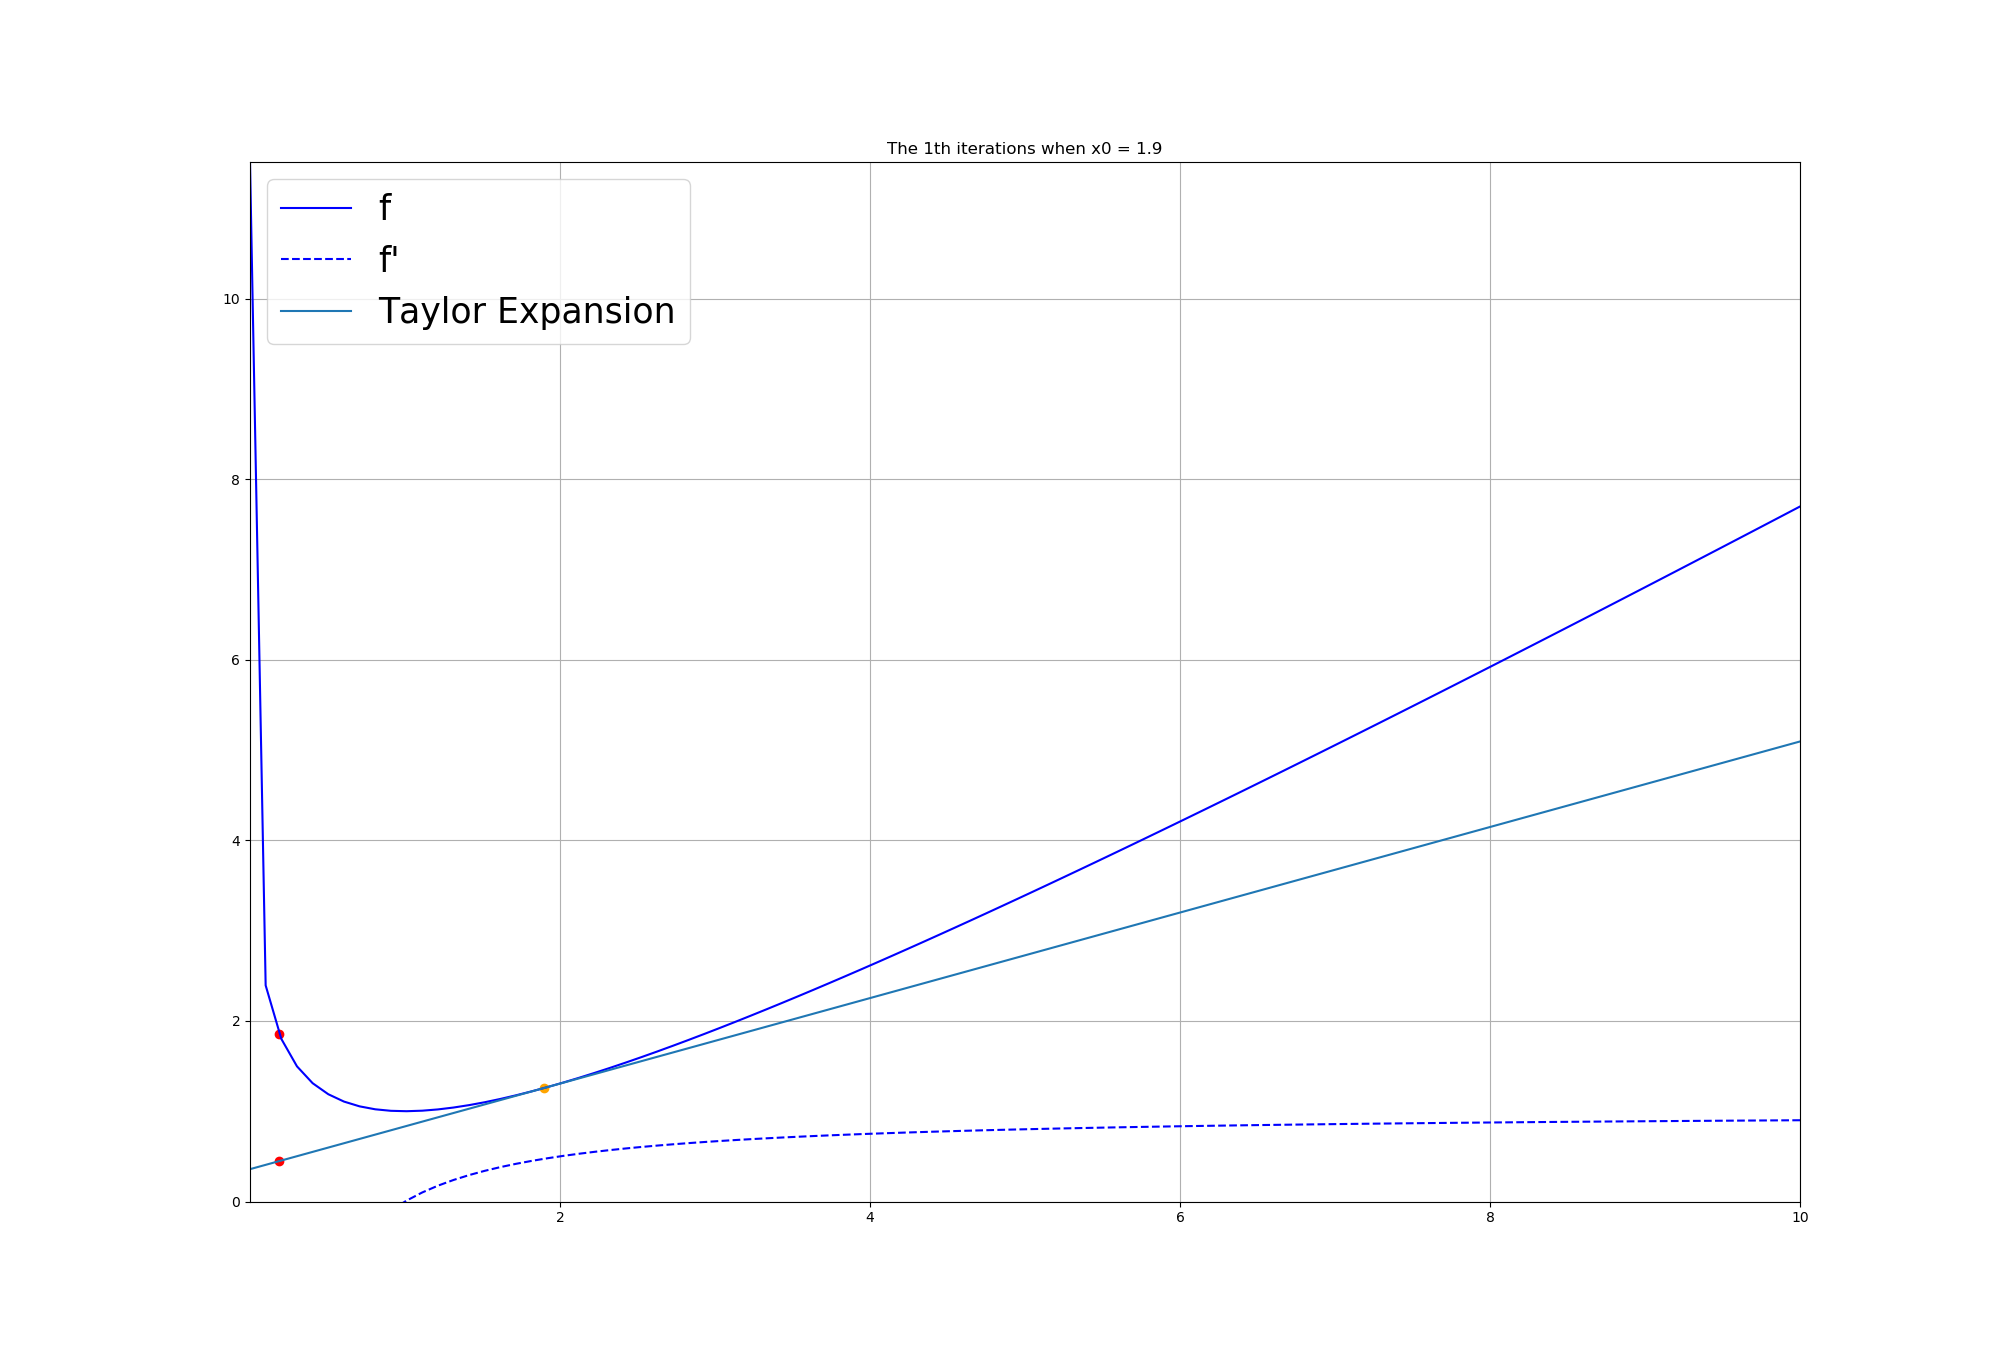
\includegraphics[scale=0.25]{f41.png}
    \end{figure}
    \begin{figure}[H]
        \centering
        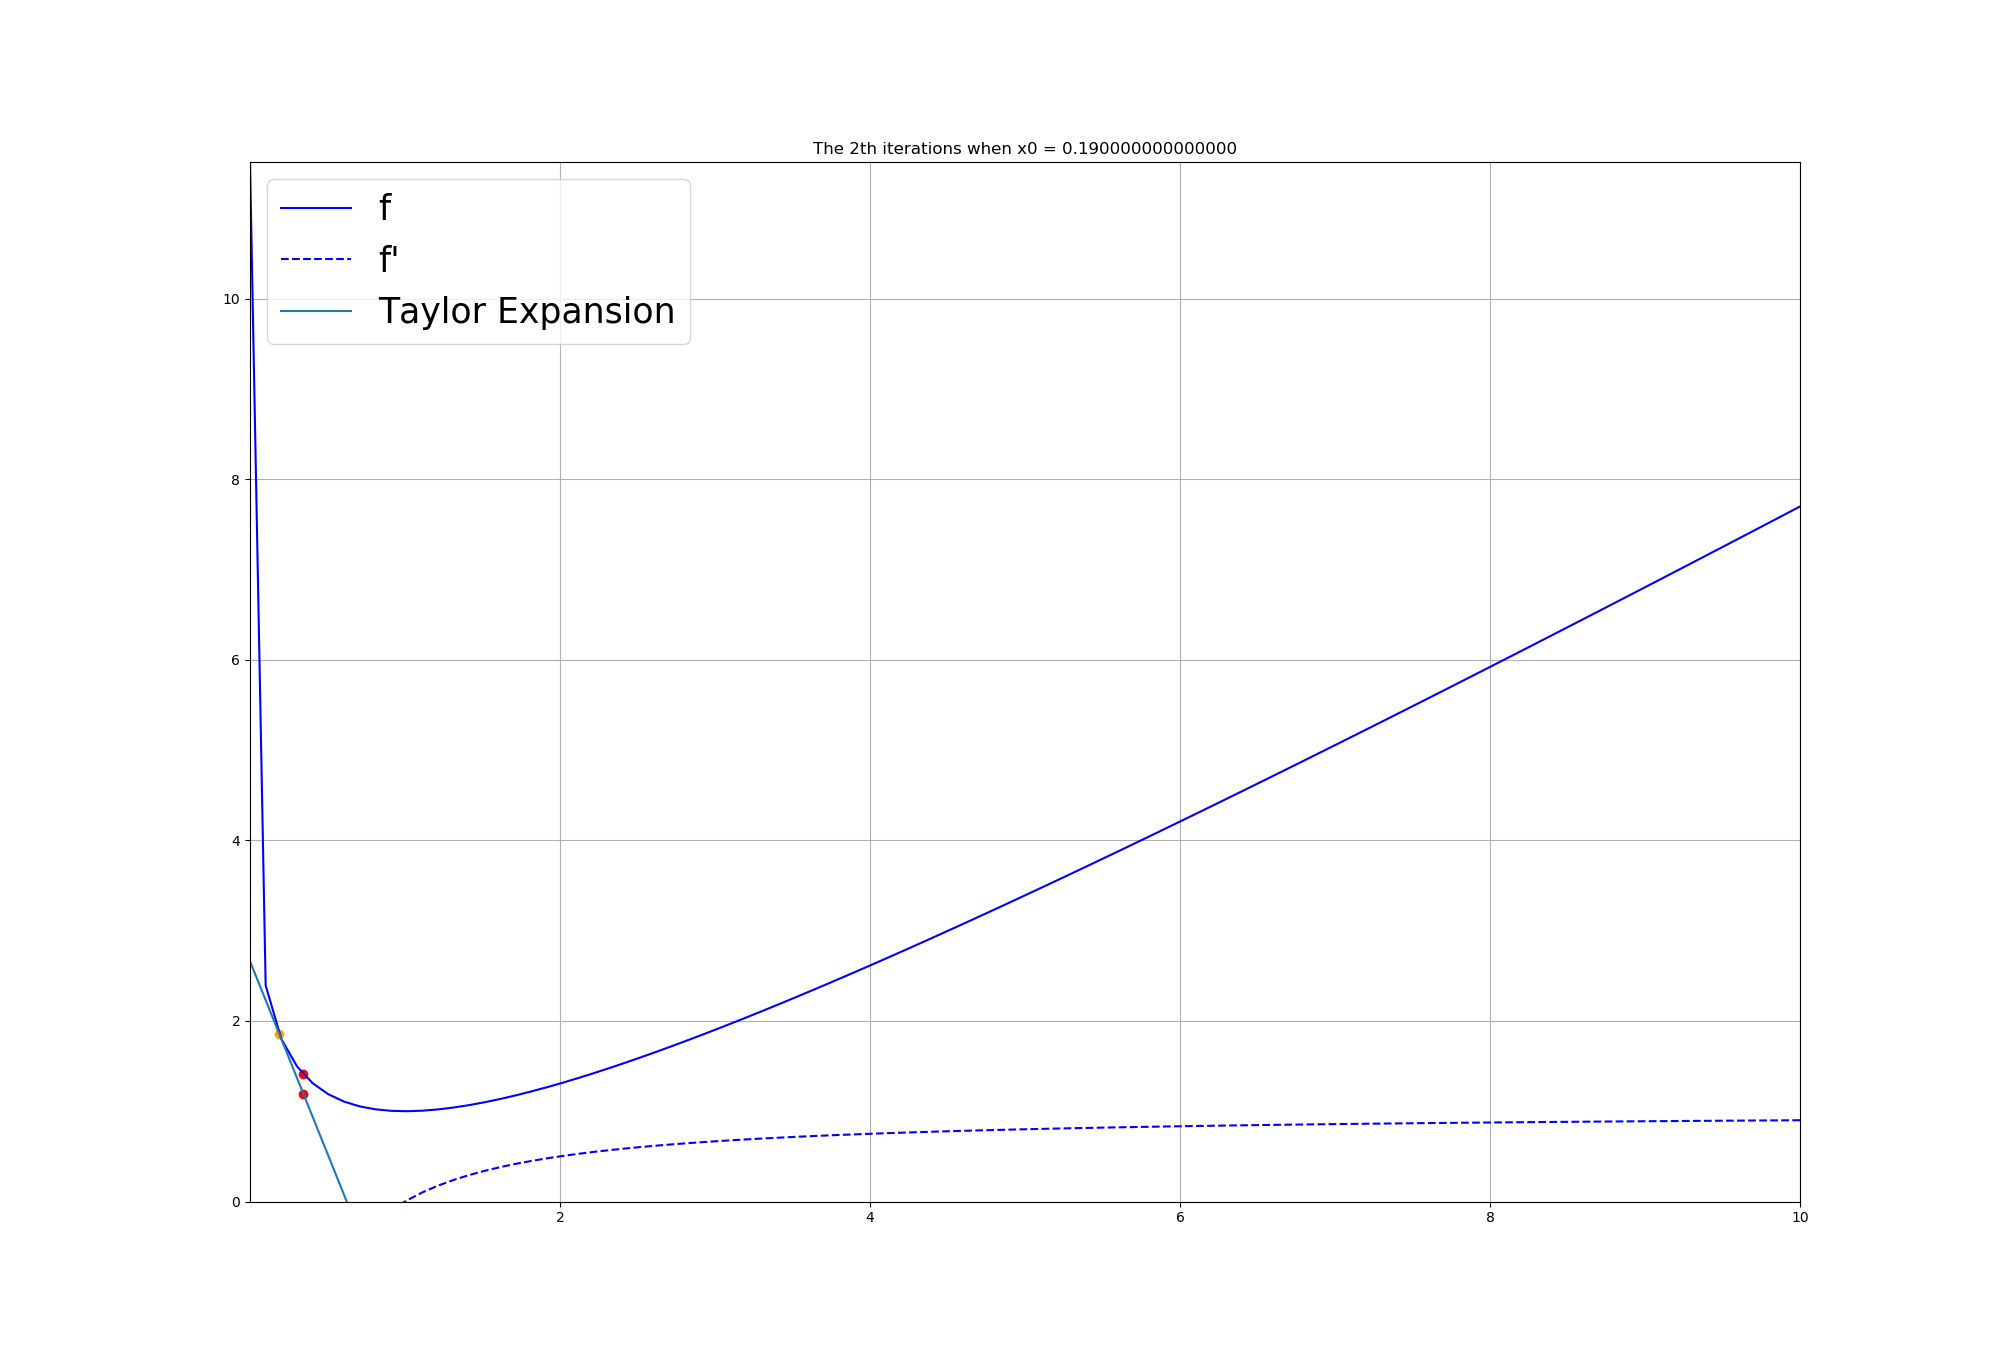
\includegraphics[scale=0.25]{f42.png}
    \end{figure}
    \begin{figure}[H]
        \centering
        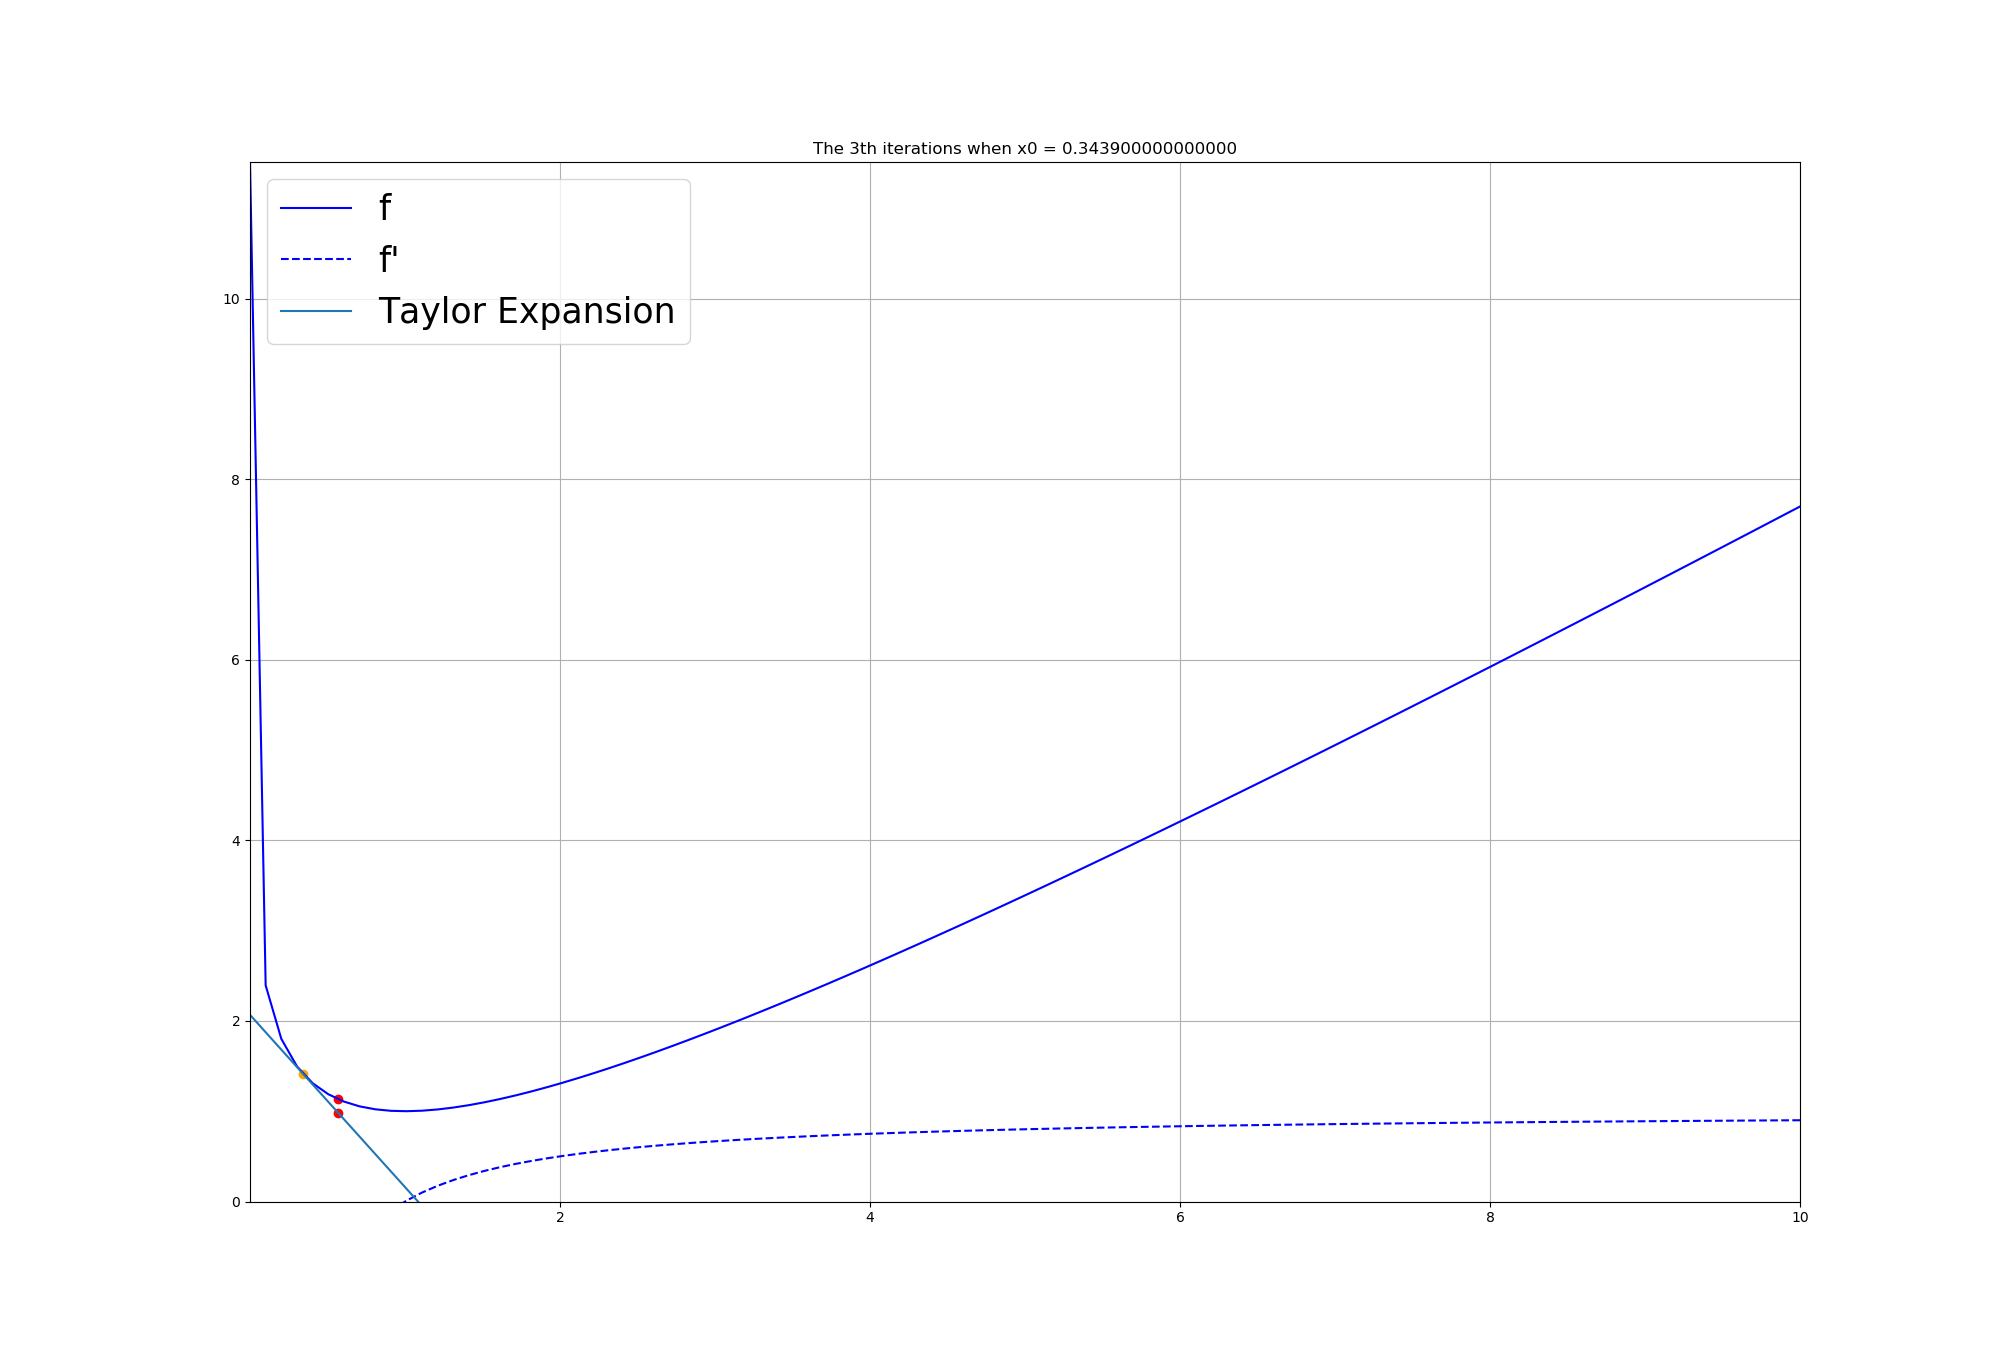
\includegraphics[scale=0.25]{f43.png}
    \end{figure}
    \begin{figure}[H]
        \centering
        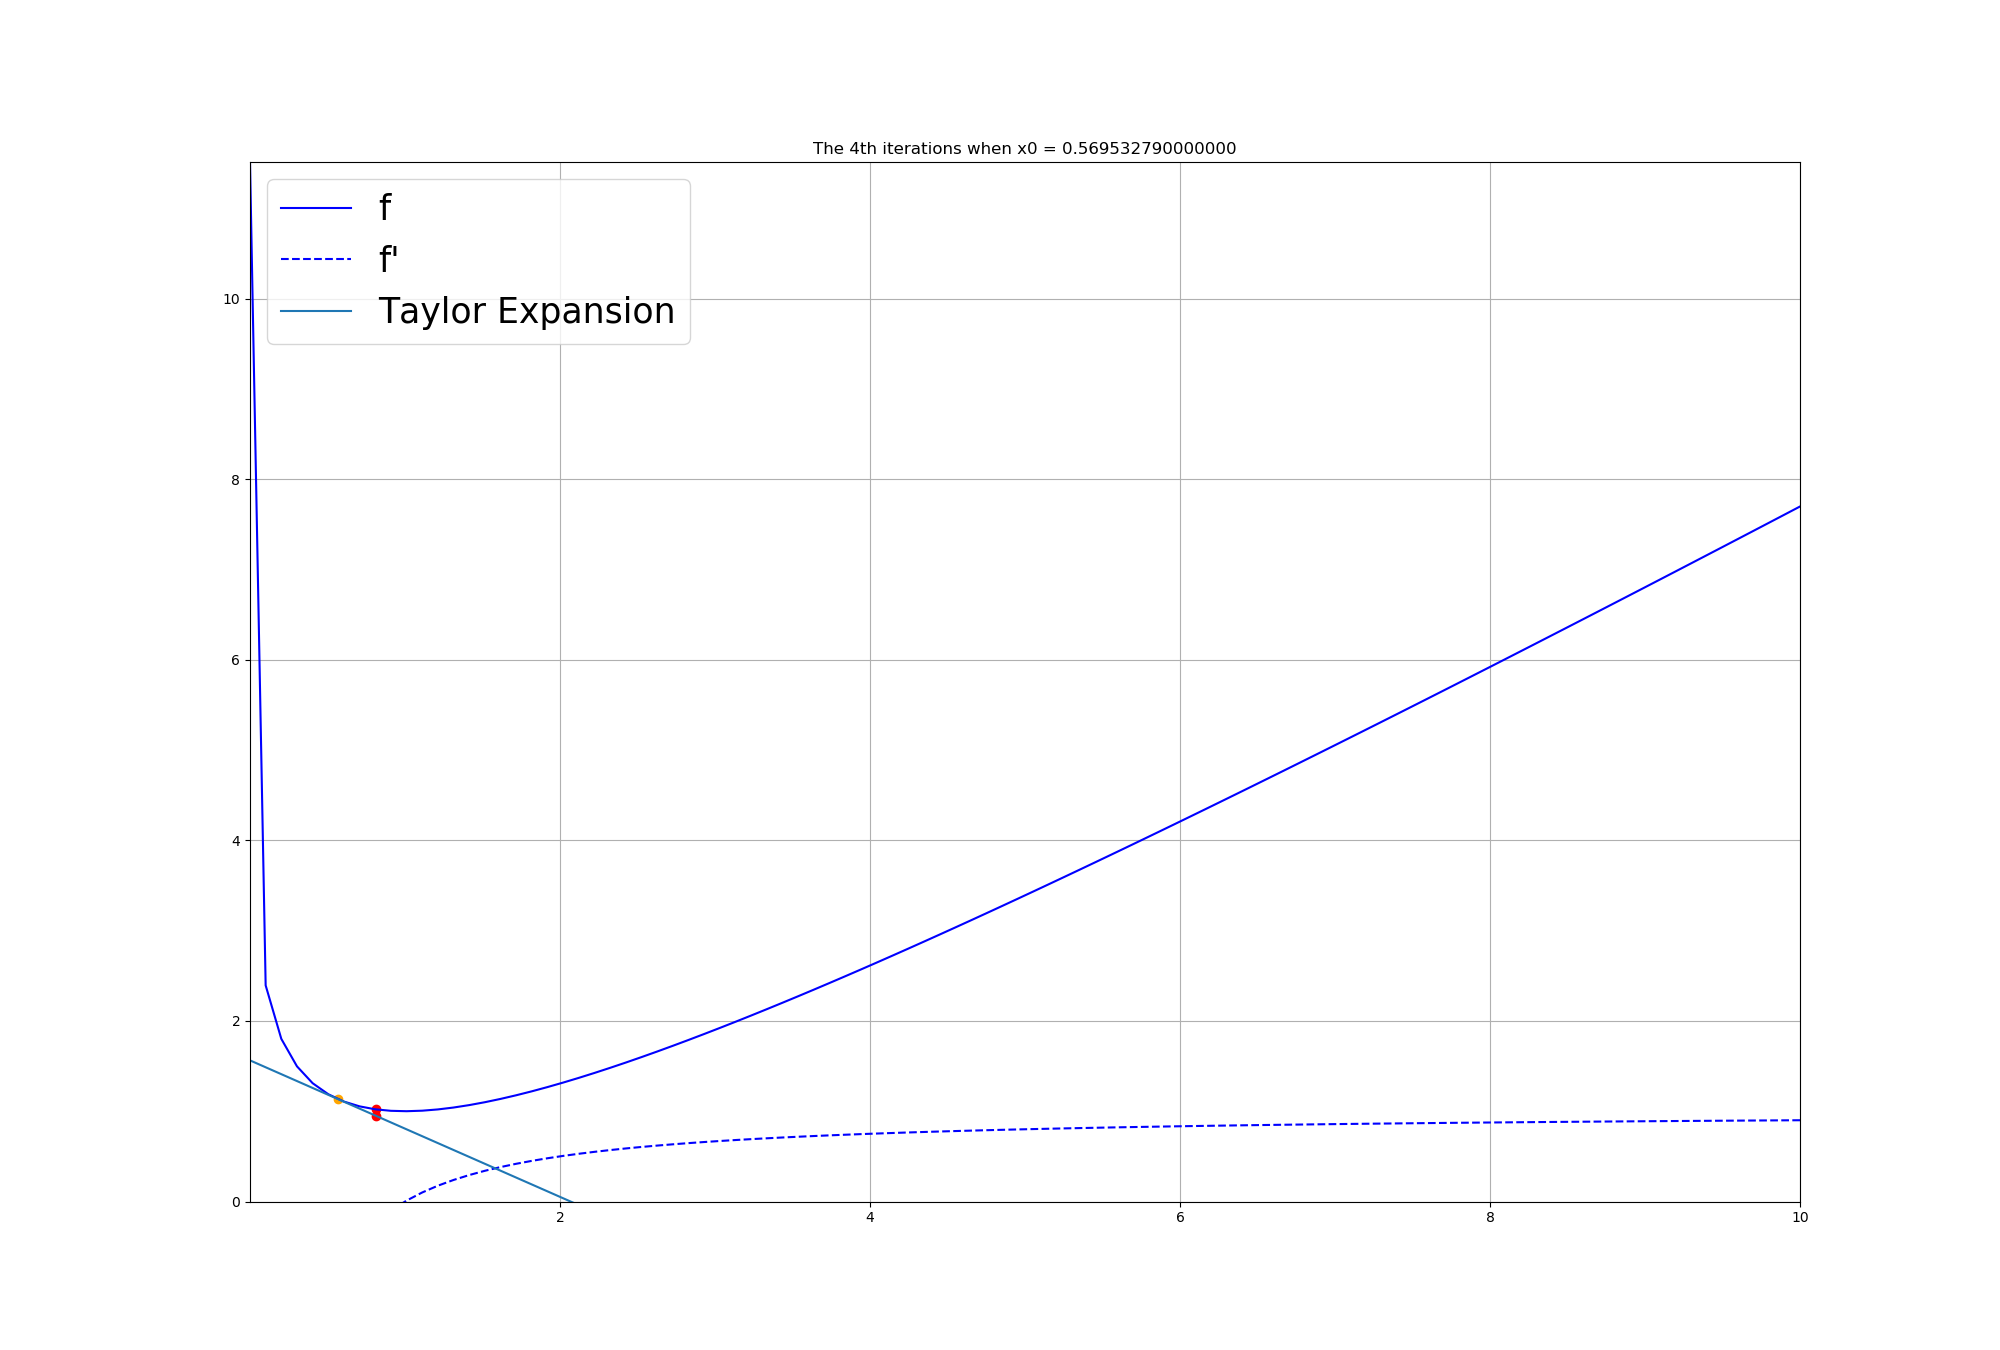
\includegraphics[scale=0.25]{f44.png}
    \end{figure}
    \begin{figure}[H]
        \centering
        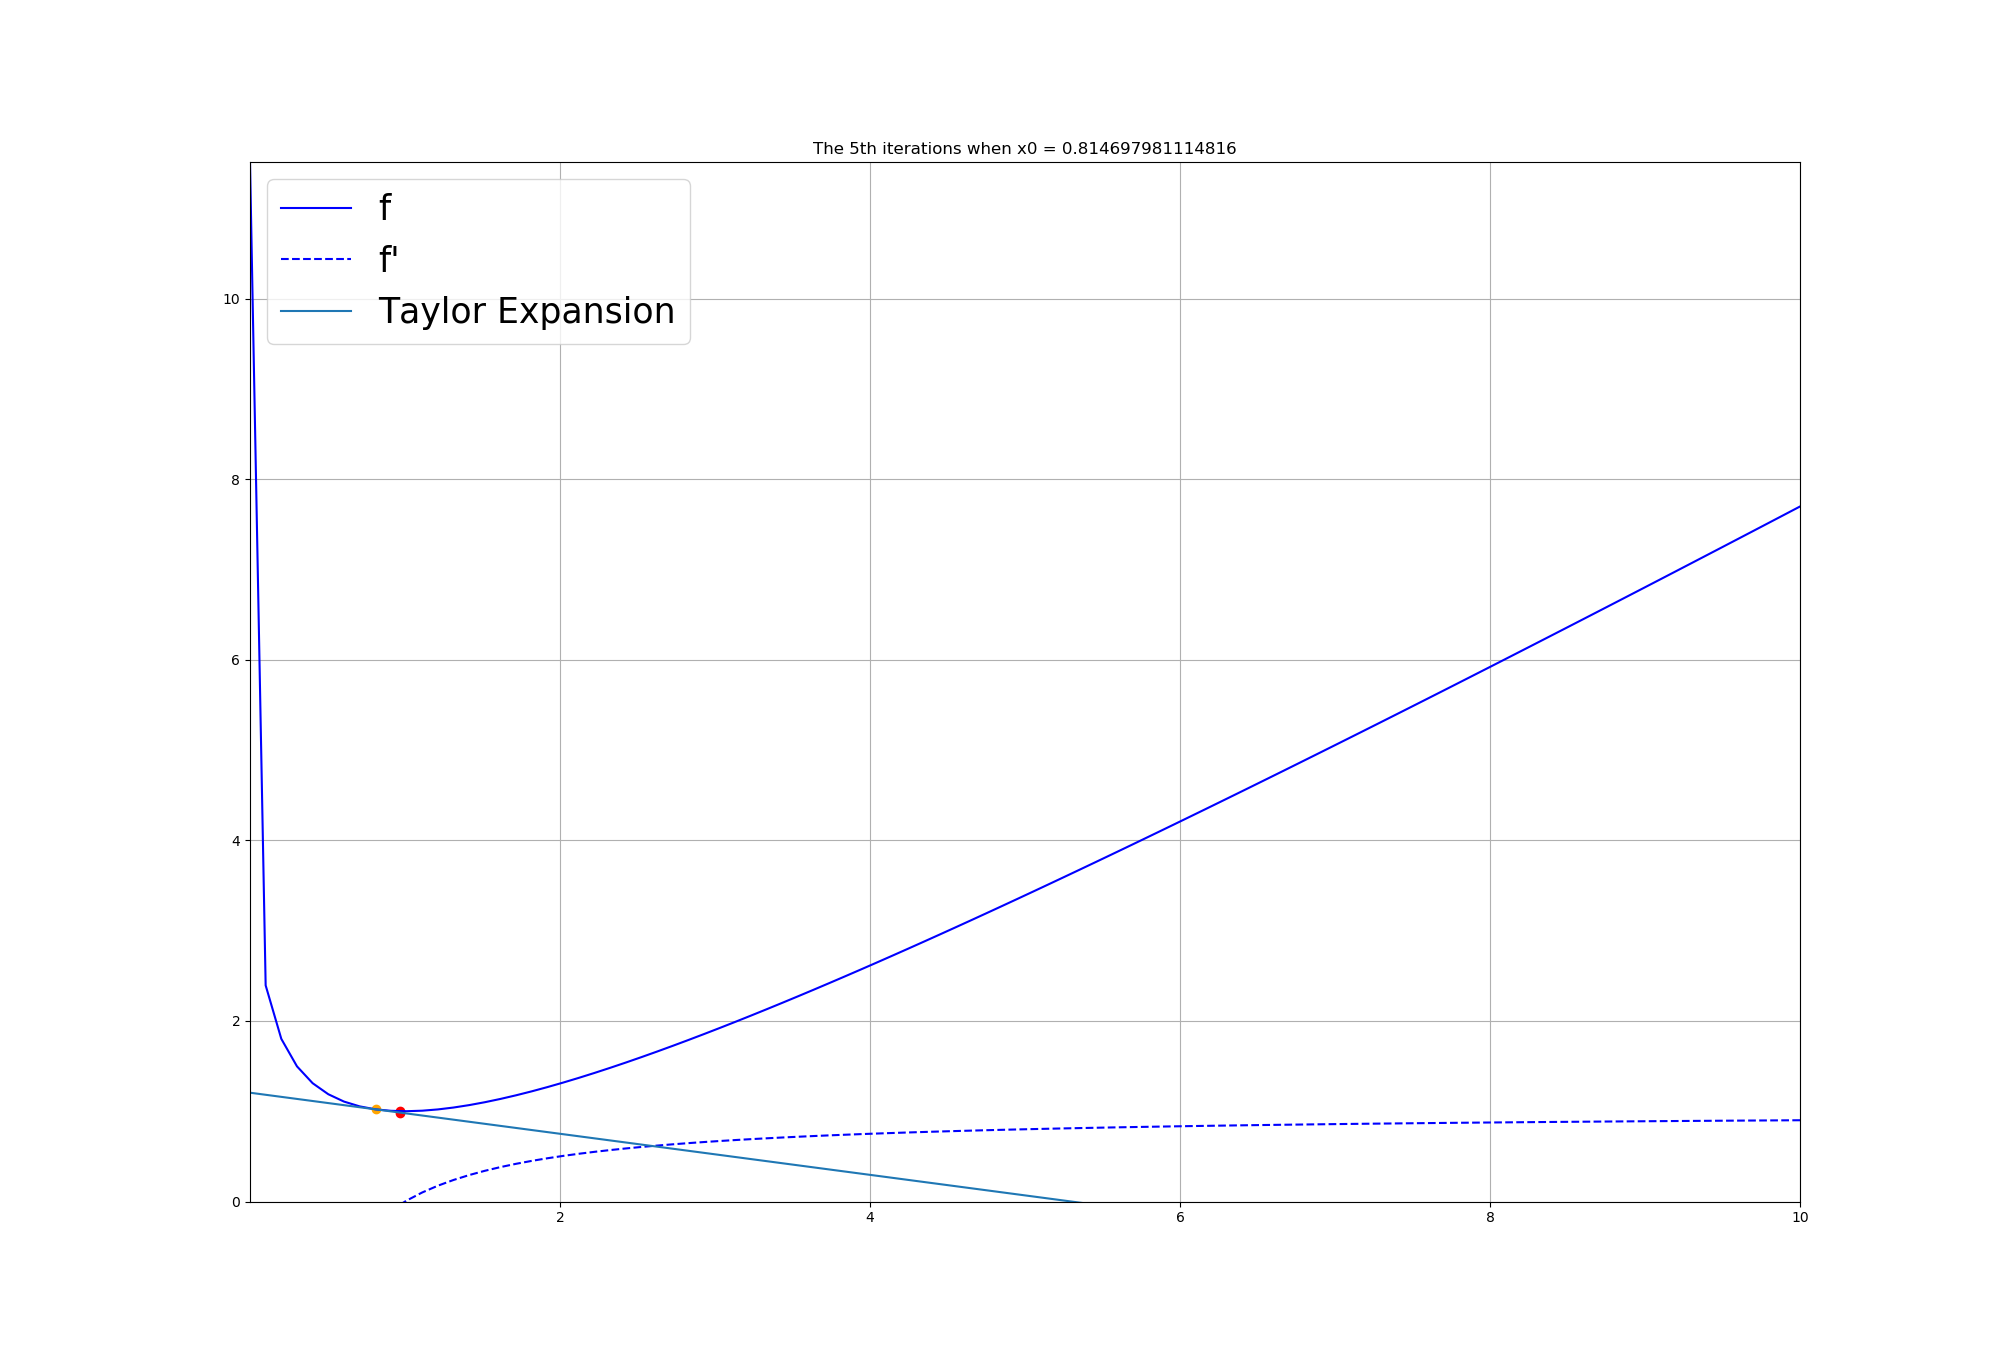
\includegraphics[scale=0.25]{f45.png}
    \end{figure}
    \begin{figure}[H]
        \centering
        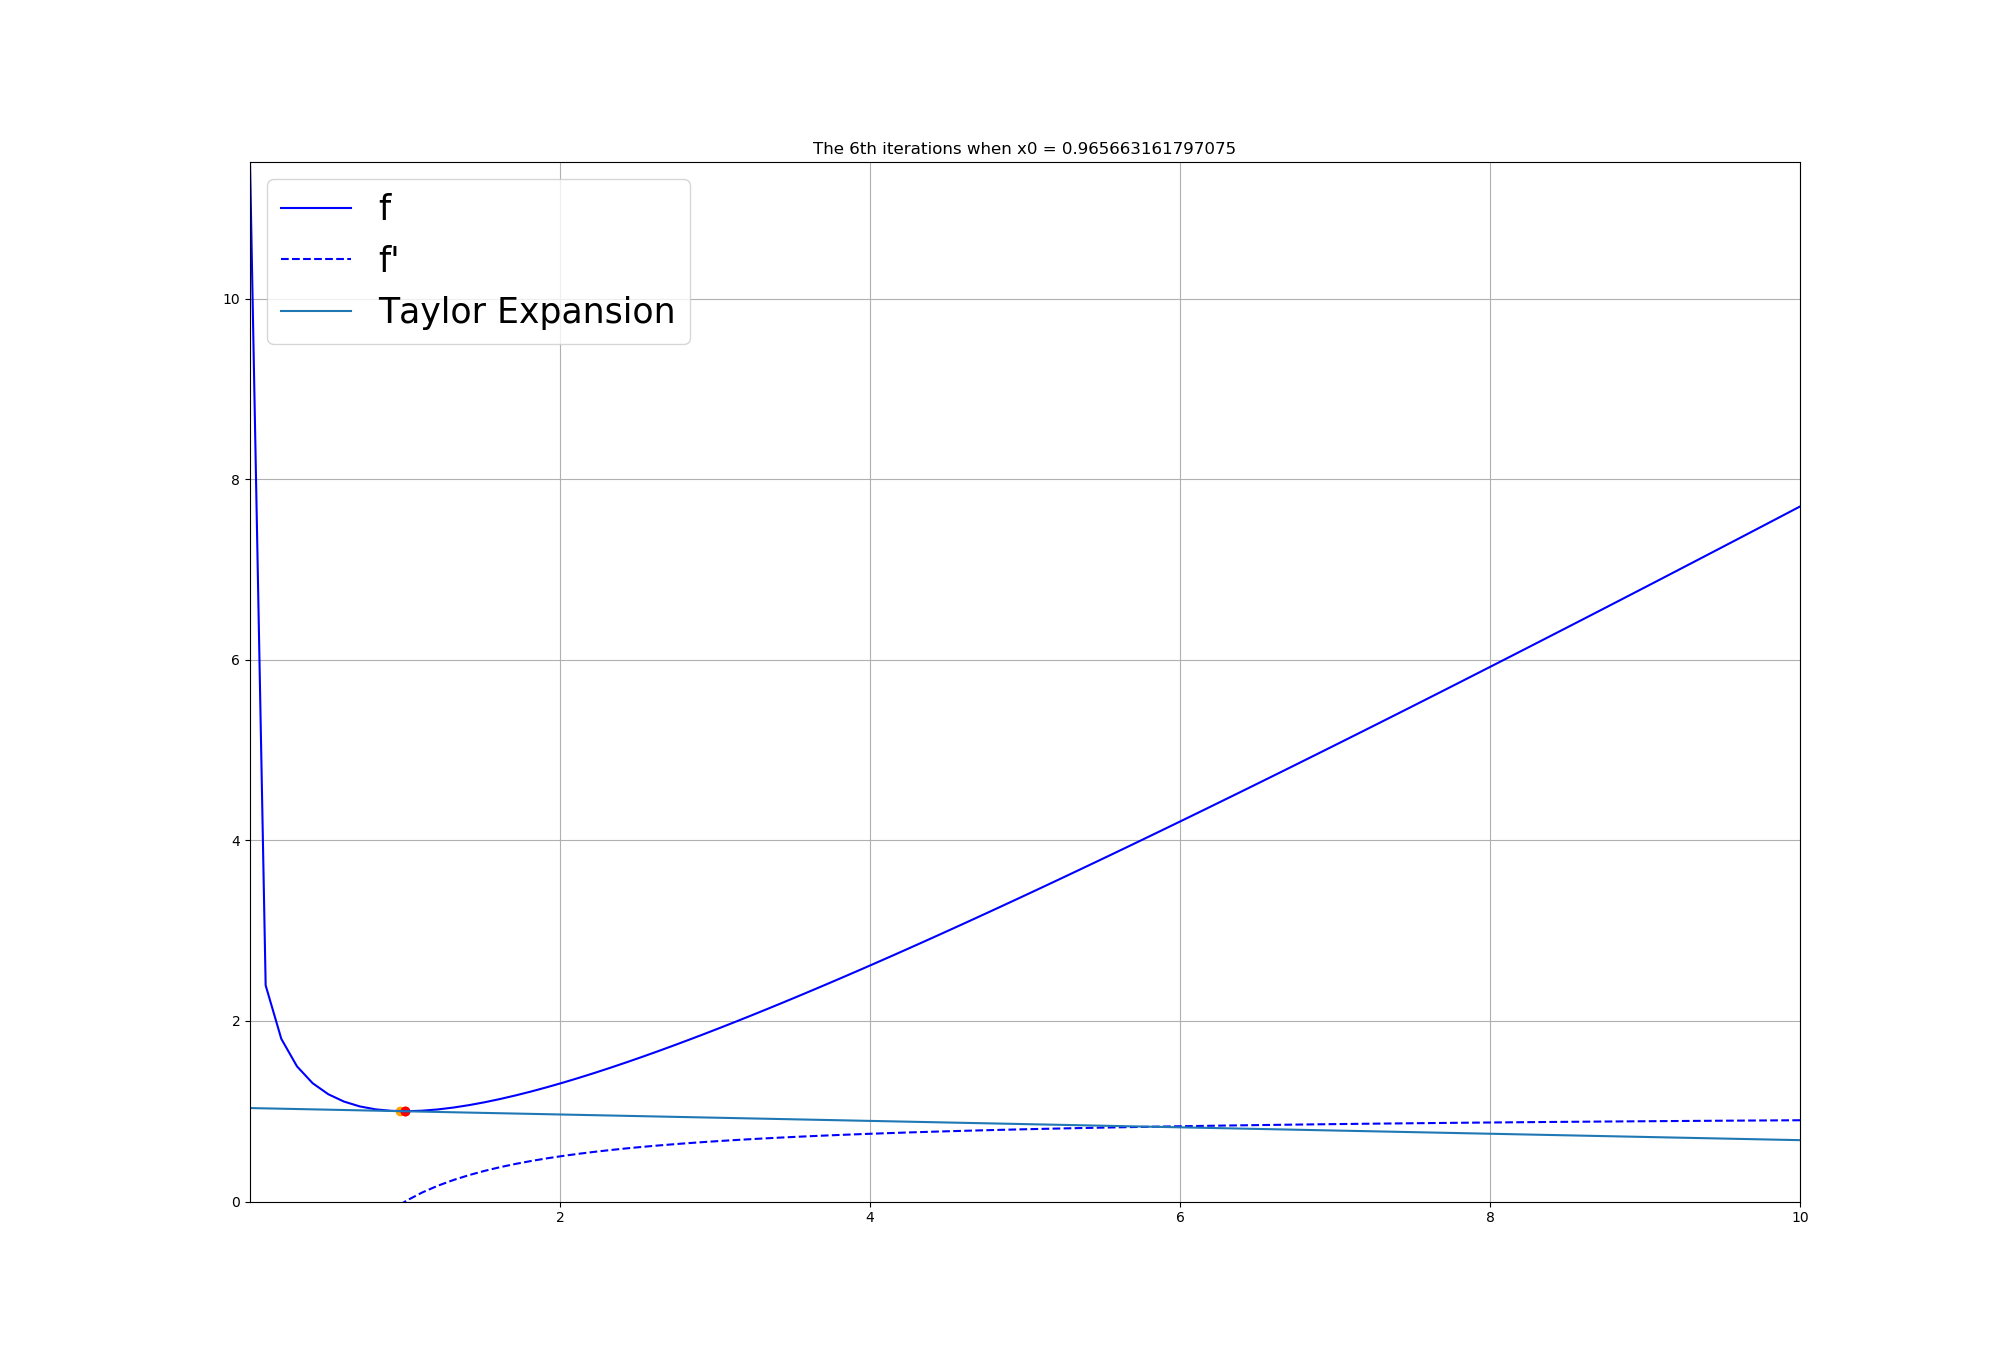
\includegraphics[scale=0.25]{f46.png}
    \end{figure}
    \begin{figure}[H]
        \centering
        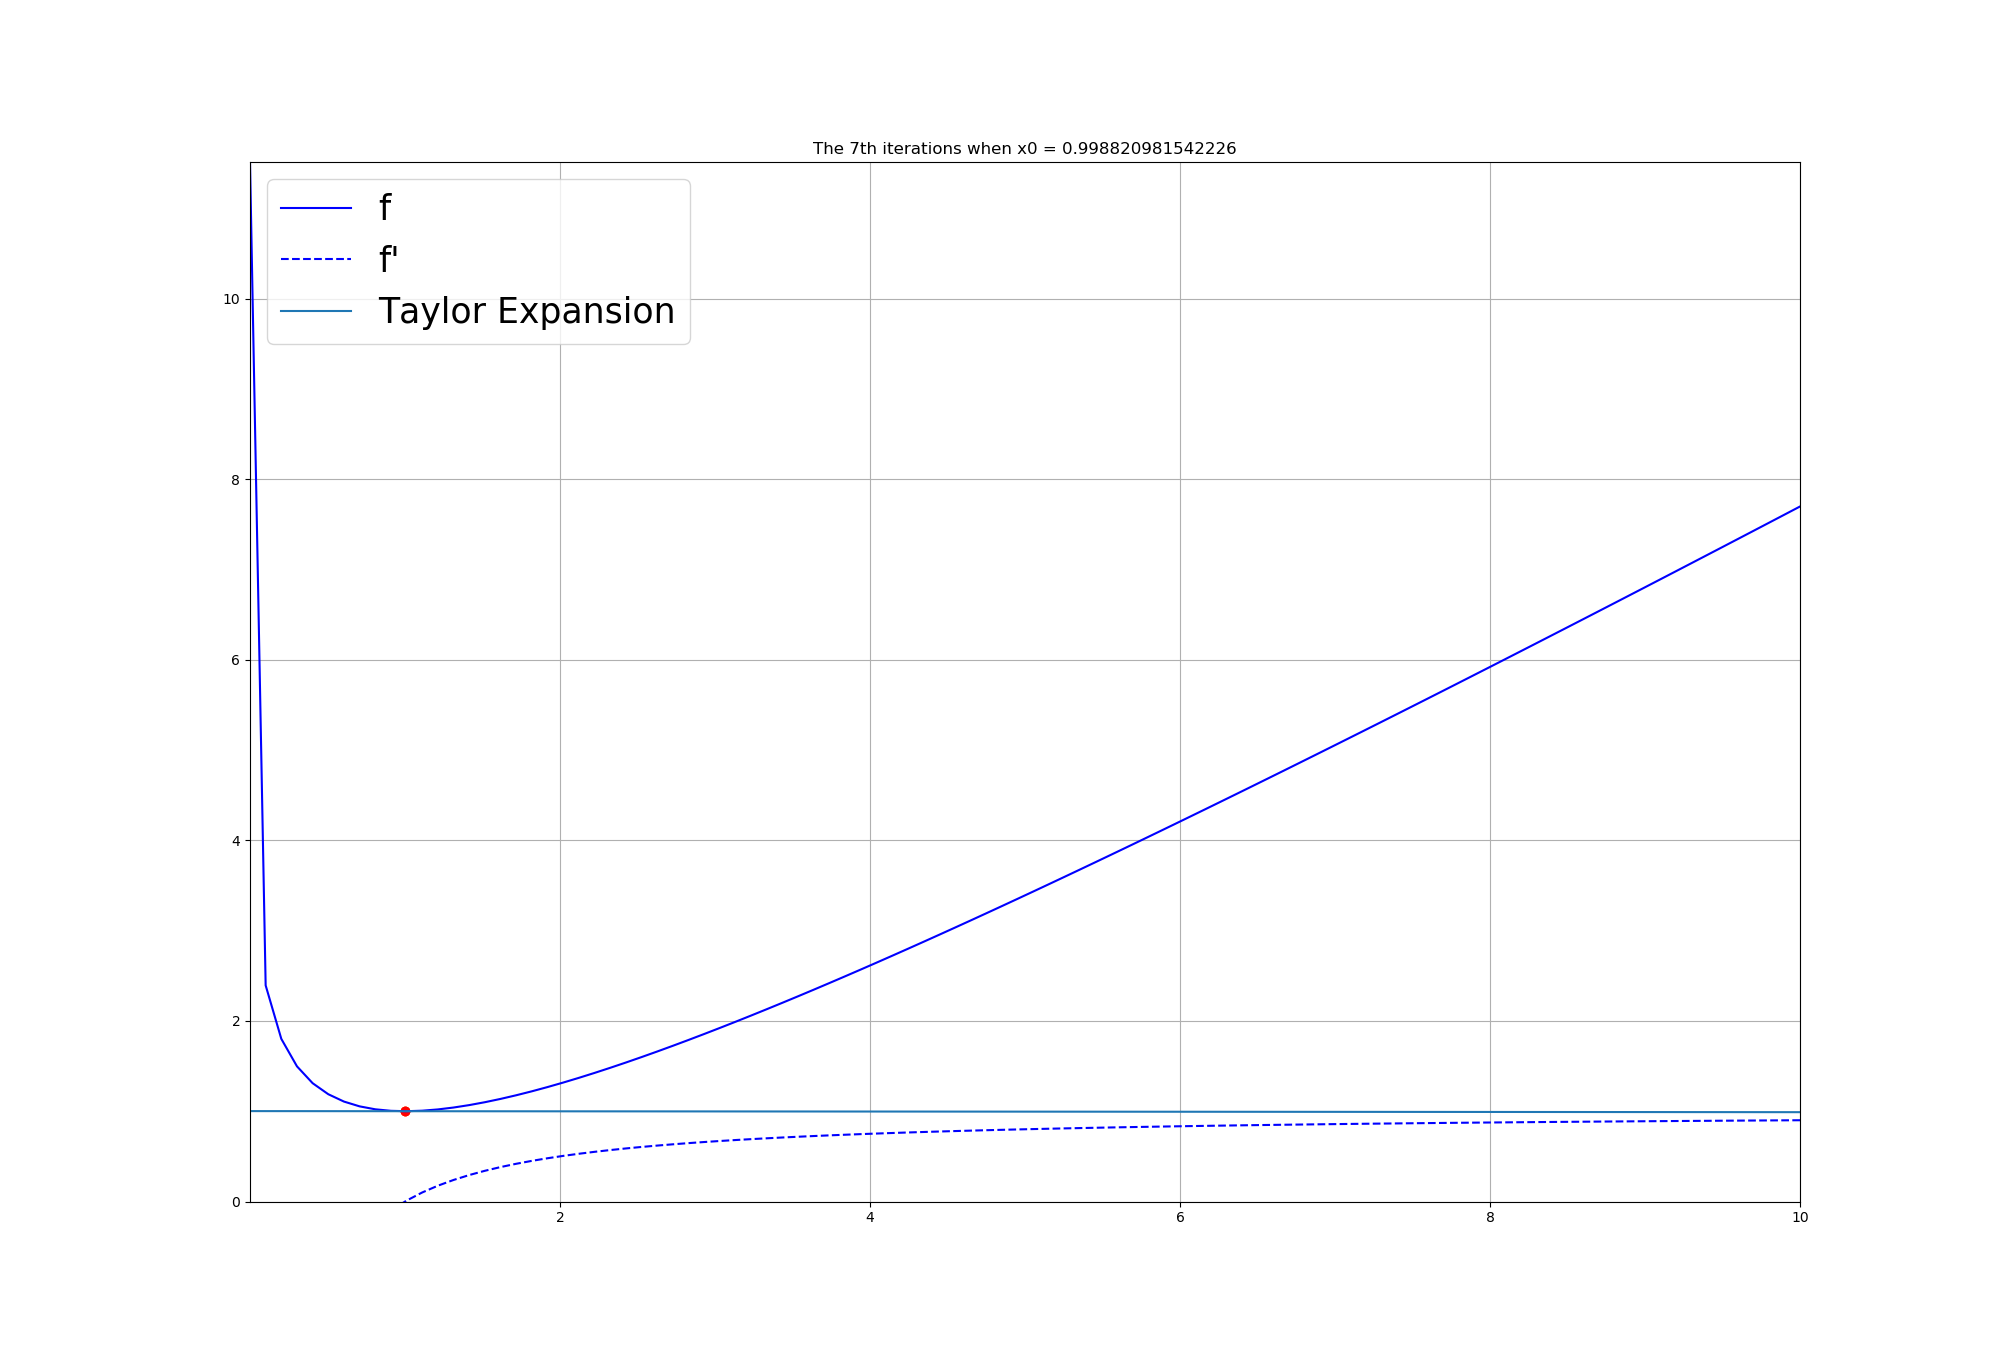
\includegraphics[scale=0.25]{f47.png}
    \end{figure}
    Therefore, according to my observation, for the \textbf{\emph{Pure Newton Method}} where $t$ is constant, the closer $x$ to the minimize point, the more possible it's going to converge. In our two cases, the converge distance both happen to be 1. 
\end{enumerate}

%%%%%%%%%%%%%%%%%%%%%%%%%%%%%%%%%%%%%%%%%%%%%%%%%%%%%%%%%%%%%%%%%%%%
% Reference
%%%%%%%%%%%%%%%%%%%%%%%%%%%%%%%%%%%%%%%%%%%%%%%%%%%%%%%%%%%%%%%%%%%%
\section*{P1 Python Code}
    \begin{verbatim}
        from sympy import *
        import numpy as np
        import matplotlib.pyplot as plt
        x = Symbol('x')
        fx = log(exp(x)+exp(-x))
        # fx = -log(x) + x
        t = 1
        x0 = 3
        fdx = diff(fx,x)
        fddx = diff(fdx,x)
        e = 1e-5
        k=1
        while 1 :
        
            tx = fx.subs(x,x0)+fdx.subs(x,x0)*(x-x0)+fddx.subs(x,x0)*(x0-x0)**2/2
            x_nt = -fdx.evalf(subs = {'x':x0})/fddx.evalf(subs = {'x':x0})
            l=(x_nt**2)**0.5
            plt.figure(figsize=(20,20))
            plt.grid(1)
            # draw the points
            plt.scatter(x0,fx.evalf(subs = {'x':x0}),color='orange')
            title='The ' + str(k) + 'th iterations when x0 = ' + str(x0)
            x0 = x0+t*x_nt
            plt.scatter(x0,fx.evalf(subs = {'x':x0}),color='red')
            plt.scatter(x0,tx.evalf(subs = {'x':x0}),color='red')
            # draw the graph of functions
            n = np.linspace(float(x0)-5,float(x0)+5,100)
            Tx=[]
            Fx=[]
            Fdx=[]
            for i in range(len(n)) :
                Tx.append(tx.subs(x,n[i]))
                Fx.append(fx.subs(x,n[i]))
                Fdx.append(fdx.subs(x,n[i]))
            plt.plot(n, Fx, color='blue', label='f')
            plt.plot(n, Fdx, color='blue', label="f'", linestyle='--')
            plt.plot(n, Tx, label="Taylor Expansion")
            plt.legend(loc='upper left', fontsize=25) 
            print(n)
            plt.title(title)
            plt.show()

            if l**2/2 <= e:
                break
            k=k+1
    \end{verbatim}
\section*{P2 Python Code}
    \begin{verbatim}
        from sympy import *
        import numpy as np
        import matplotlib.pyplot as plt
        x = Symbol('x')
        # fx = log(exp(x)+exp(-x))
        fx = -log(x) + x
        t = 1
        x0 = 3
        fdx = diff(fx,x)
        fddx = diff(fdx,x)
        e = 1e-5
        k=1
        while 1 :
        
            tx = fx.subs(x,x0)+fdx.subs(x,x0)*(x-x0)+fddx.subs(x,x0)*(x0-x0)**2/2
            x_nt = -fdx.evalf(subs = {'x':x0})/fddx.evalf(subs = {'x':x0})
            l=(x_nt**2)**0.5
            plt.figure(figsize=(20,20))
            plt.grid(1)
            # draw the points
            plt.scatter(x0,fx.evalf(subs = {'x':x0}),color='orange')
            title='The ' + str(k) + 'th iterations when x0 = ' + str(x0)
            x0 = x0+t*x_nt
            plt.scatter(x0,fx.evalf(subs = {'x':x0}),color='red')
            plt.scatter(x0,tx.evalf(subs = {'x':x0}),color='red')
            # draw the graph of functions
            left=float(x0)-5
            right=float(x0)+5
            if left<=0:
                left=1e-5
                right=left+10
            n = np.linspace(left,right,100)
            Tx=[]
            Fx=[]
            Fdx=[]
            for i in range(len(n)) :
                Tx.append(tx.subs(x,n[i]))
                Fx.append(fx.subs(x,n[i]))
                Fdx.append(fdx.subs(x,n[i]))
            plt.plot(n, Fx, color='blue', label='f')
            plt.plot(n, Fdx, color='blue', label="f'", linestyle='--')
            plt.plot(n, Tx, label="Taylor Expansion")
            plt.legend(loc='upper left', fontsize=25) 
            plt.axis([left,right,0,float(max(Fx))])
            plt.title(title)
            plt.show()
            if l**2/2 <= e:
                break
            k=k+1

    \end{verbatim}
\end{document}
